 \documentclass[12pt, dvipdfmx]{beamer}

\renewcommand{\kanjifamilydefault}{\gtdefault}
%%%%%%%%%%%  package  %%%%%%%%%%%
\usepackage{bxdpx-beamer}% dvipdfmxなので必要
\usepackage{pxjahyper}% 日本語で'しおり'したい

\usepackage{amssymb,amsmath,ascmac}

\usepackage{multirow}
\usepackage{bm}

\graphicspath{{../../_Figures//}{../../_Figures/Rheology/}}

\usepackage{tikz}
\usepackage{xparse}

\usetikzlibrary{shapes,arrows}
%% define fancy arrow. \tikzfancyarrow[<option>]{<text>}. ex: \tikzfancyarrow[fill=red!5]{hoge}
\tikzset{arrowstyle/.style n args={2}{inner ysep=0.1ex, inner xsep=0.5em, minimum height=2em, draw=#2, fill=black!20, font=\sffamily\bfseries, single arrow, single arrow head extend=0.4em, #1,}}
\NewDocumentCommand{\tikzfancyarrow}{O{fill=black!20} O{none}  m}{
\tikz[baseline=-0.5ex]\node [arrowstyle={#1}{#2}] {#3 \mathstrut};}

%目次スライド
\AtBeginSection[]{
  \frame{\tableofcontents[currentsection]}
}

%アペンディックスのページ番号除去
\newcommand{\backupbegin}{
   \newcounter{framenumberappendix}
   \setcounter{framenumberappendix}{\value{framenumber}}
}
\newcommand{\backupend}{
   \addtocounter{framenumberappendix}{-\value{framenumber}}
   \addtocounter{framenumber}{\value{framenumberappendix}} 
}

%%%%%%%%%%%  theme  %%%%%%%%%%%
\usetheme{Copenhagen}
% \usetheme{Metropolis}
% \usetheme{CambridgeUS}
% \usetheme{Berlin}

%%%%%%%%%%%  inner theme  %%%%%%%%%%%
% \useinnertheme{default}

% %%%%%%%%%%%  outer theme  %%%%%%%%%%%
\useoutertheme{default}
% \useoutertheme{infolines}

%%%%%%%%%%%  color theme  %%%%%%%%%%%
%\usecolortheme{structure}

%%%%%%%%%%%  font theme  %%%%%%%%%%%
\usefonttheme{professionalfonts}
%\usefonttheme{default}

%%%%%%%%%%%  degree of transparency  %%%%%%%%%%%
%\setbeamercovered{transparent=30}

% \setbeamertemplate{items}[default]

%%%%%%%%%%%  numbering  %%%%%%%%%%%
% \setbeamertemplate{numbered}
\setbeamertemplate{navigation symbols}{}
\setbeamertemplate{footline}[frame number]


\title
[粘弾性の基礎]
{粘弾性の基礎}
\author[東亞合成 佐々木]{佐々木 裕\thanks{hiroshi\_sasaki@mail.toagosei.co.jp}}
\institute[東亞合成]{東亞合成株式会社}
\date{}

\begin{document}

%%%%%
% 1 P
%%%%%
\maketitle

%%%%%
% 2 P
%%%%%
%% 目次 (必要なければ省略)
\begin{frame}
\frametitle{Outline}
\tableofcontents
\end{frame}

\begin{frame}
	\frametitle{この章でのお話}
	この章では、いよいよレオロジーの主たる対象である粘性と弾性を併せ持った粘弾性という性質についてです。
		\begin{boxnote}
			\vspace{-3mm}
			\begin{itemize}
				\item 粘性と弾性についての再確認
					\begin{itemize}
						\item 固体と液体の応答について振り返り、
						\item その組み合わせとして粘弾性
					\end{itemize} 
				\item 粘弾性のモデル化
					\begin{itemize}
						\item 粘弾性の単純なモデルをつくって、
						\item 応力緩和と緩和時間
					\end{itemize} 
				\item 少しだけ実事象に近づけると
					\begin{itemize}
						\item 複数の緩和時間を一般化マックスウェルモデル
						\item 応力緩和で見た固体と液体
					\end{itemize}
			\end{itemize}
		\end{boxnote}
\end{frame}

\section{粘性と弾性についての再確認}
\subsection{固体と液体の応答について}
\begin{frame}
	\frametitle{レオロジーのやり方の再確認}
	\begin{block}{レオロジーのやり方}
		レオロジーとは、物質に刺激を与えてその応答を評価観察することで、その特性を評価できるのでした。\\
		ここでは、物質の力学的な応答である弾性と粘性について検討を進めます。
	\end{block}
	\begin{columns}[T, onlytextwidth]
		\column{.58\linewidth}
			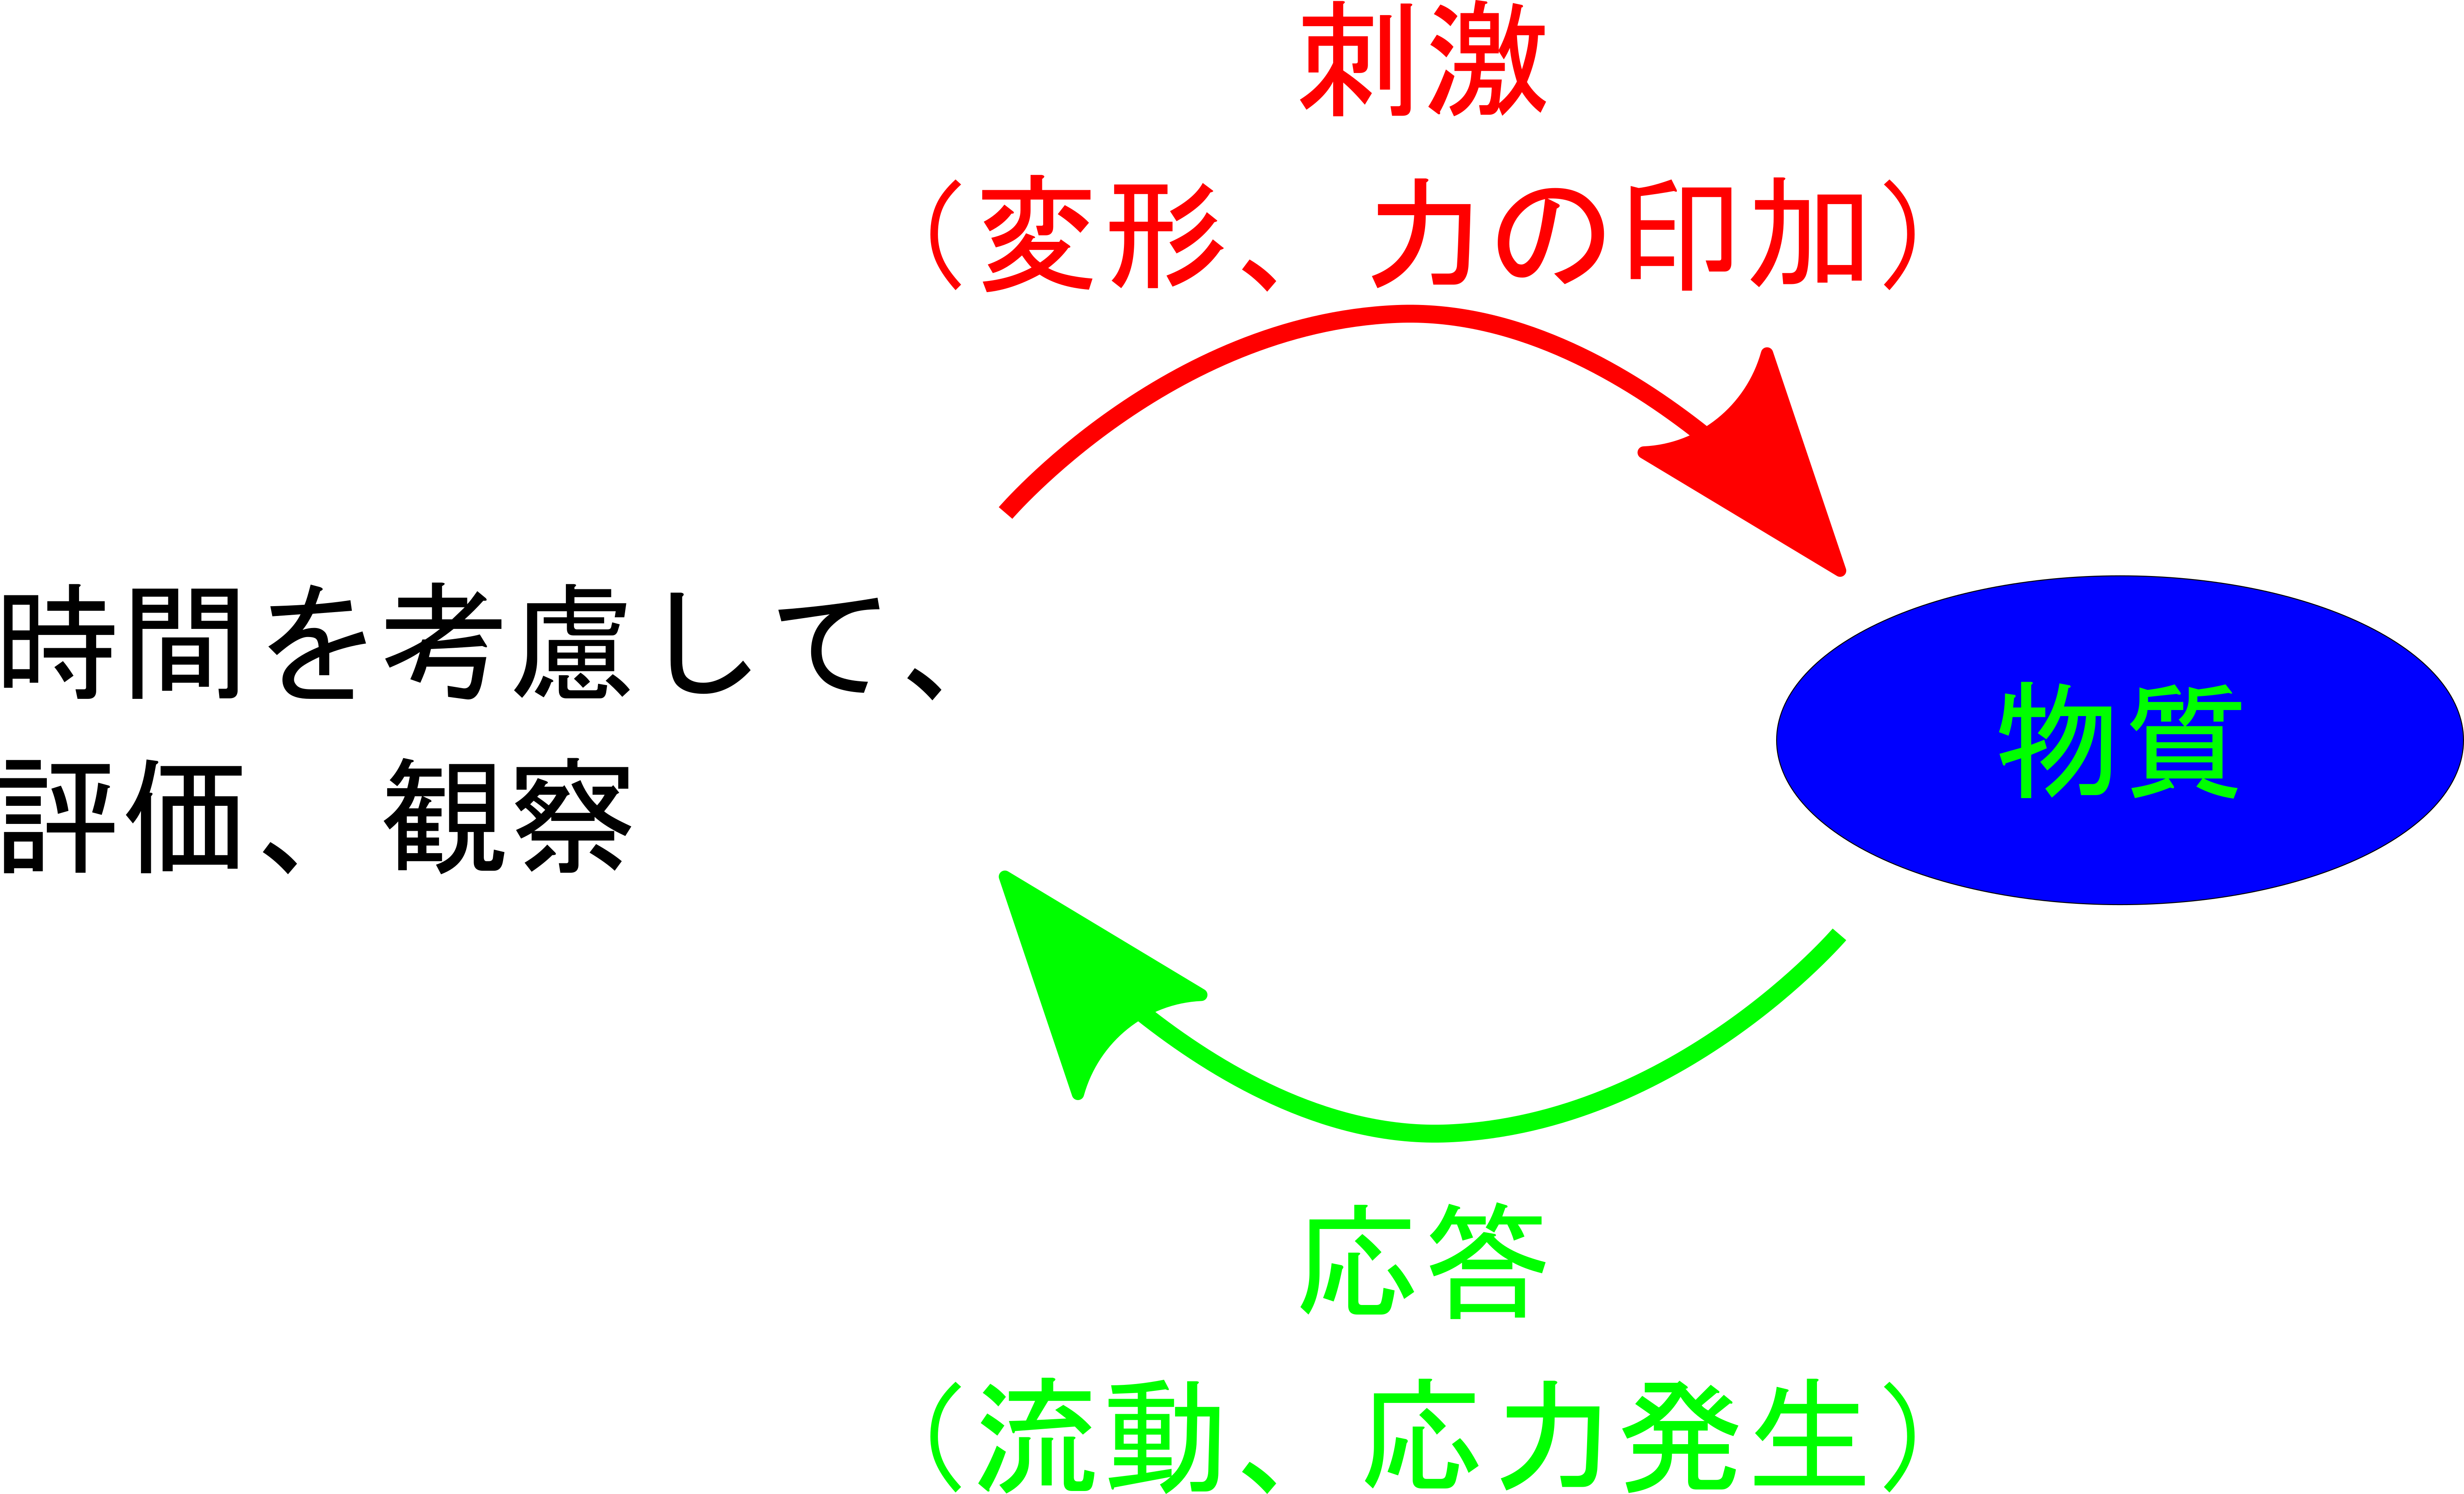
\includegraphics[width=\textwidth]{Rheo_method.png}
		\column{.38\linewidth}
			\begin{itemize}
				\item 力学的な刺激
				\begin{itemize}
					\item 外力による\\物質の変形
				\end{itemize}
				\item 変形の結果として
				\begin{itemize}
					\item 応力が発生
				\end{itemize}
				\item 弾性と粘性
			\end{itemize}
	\end{columns}
\end{frame}

\begin{frame}
	\frametitle{固体と液体の応答について}
			\begin{center}
				\begin{tabular}{|c||c|} \hline
					固体のモデル	& 液体のモデル \\ \hline \hline
					応力は\alert{ひずみに比例}	& 応力は\alert{ひずみ速度に比例}\\
					$\text{応力} = \text{弾性率} \times \text{ひずみ}$	& $\text{応力} = \text{粘度} \times \text{ひずみ速度}$ \\ \hline
					比例定数が弾性率	& 比例定数が粘度\\ 
					弾性率の単位は、[Pa]	& 粘度の単位は、[Pa$\cdot$s]\\ \hline
					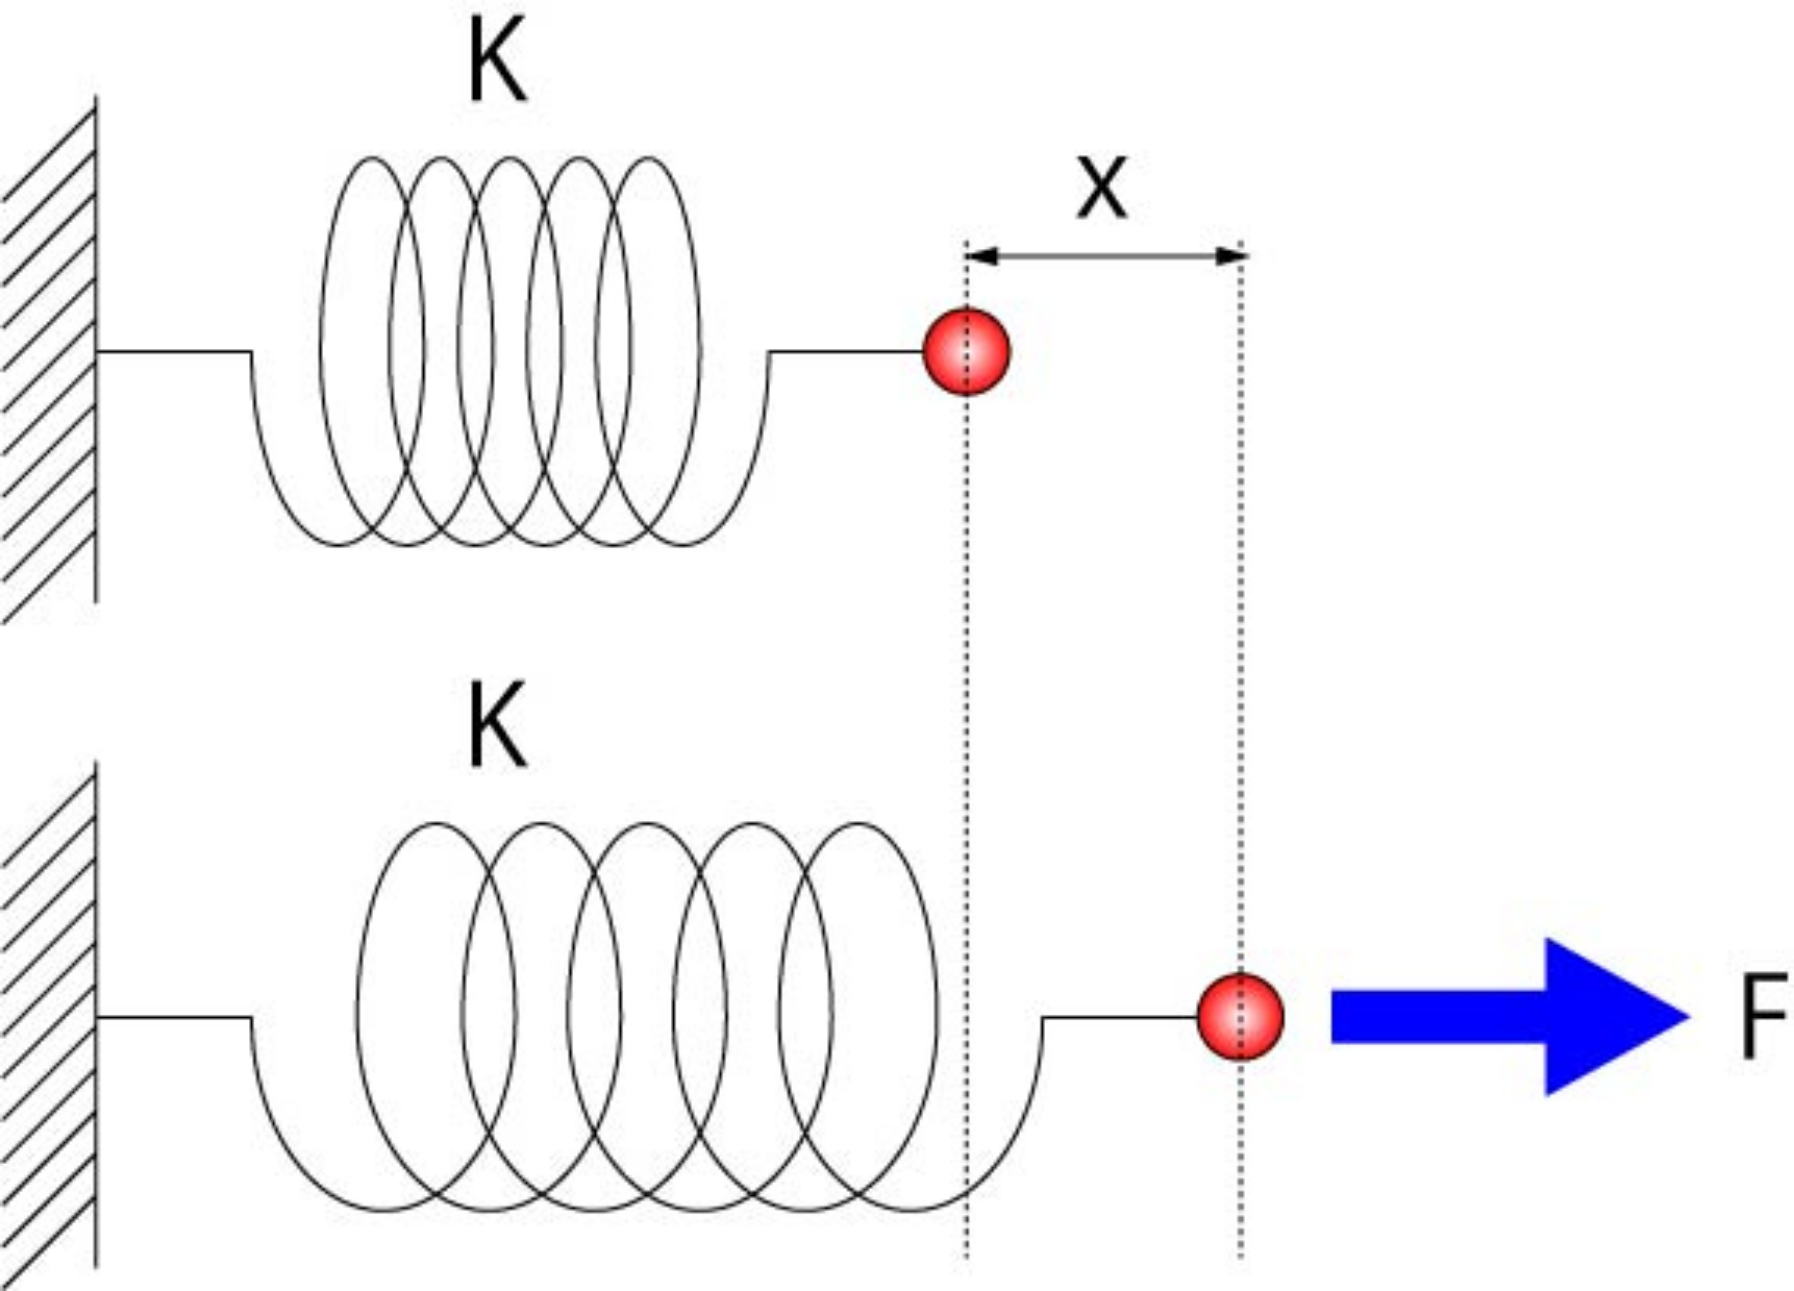
\includegraphics[width= 0.25\textwidth]{spring.png} & 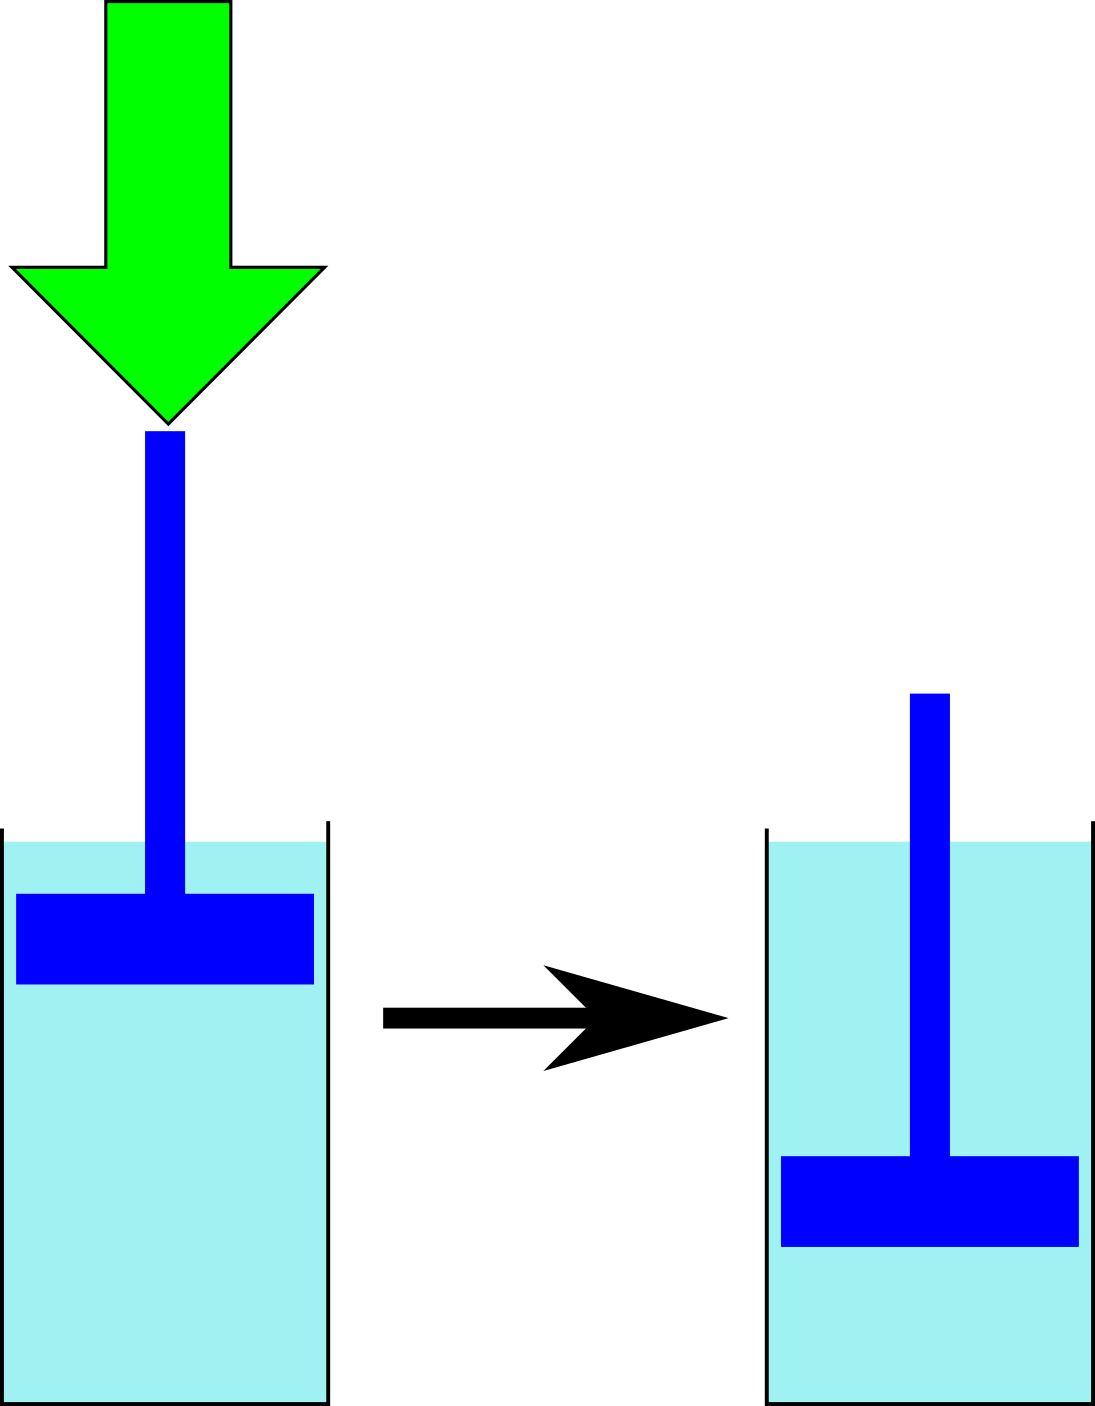
\includegraphics[width=.25\textwidth]{dashpot.png} \\ \hline
					\alert{力の釣り合い}	& 	\alert{時間の因子が重要} \\ \hline
				\end{tabular}
			\end{center}
\end{frame}

\subsection{実事象は複雑}
\begin{frame}
	\frametitle{各種の応答特性の分類}
		\begin{itemize}
			\item 図の左側が弾性応答
			\item 右側が流動特性
			\item 単純に二分されるわけでもなく、\alert{粘性と弾性を\\併せ持ったもの}が多く存在。
		\end{itemize}
			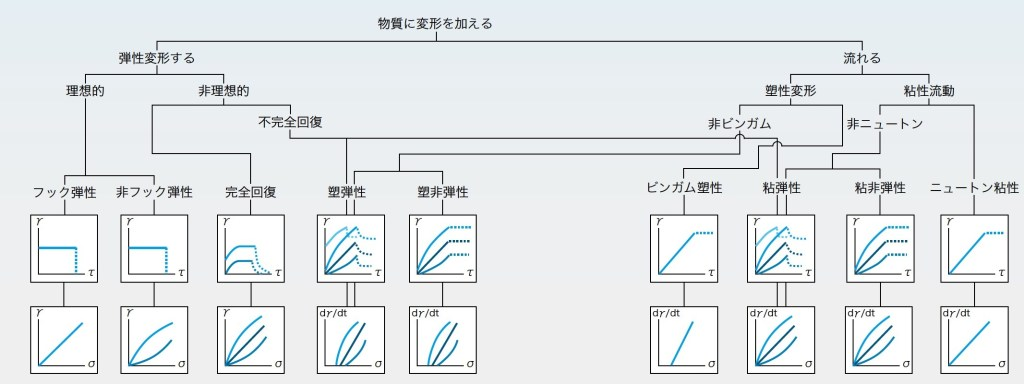
\includegraphics[width=\textwidth]{reoroji.jpeg}
			Nature 1942 v149-3790, p702
			% \href{http://rheology.jp/nagoya/2017/10/%e3%83%ac%e3%82%aa%e3%83%ad%e3%82%b8%e3%83%bc%e7%9a%84%e3%81%aa%e7%89%a9%e8%b3%aa%e3%81%ae%e5%88%86%e9%a1%9e/}{この絵のサイトへのリンク}
\end{frame}

\subsection{粘弾性について考えてみましょう}
\begin{frame}
	\frametitle{粘弾性について}
		\begin{block}{粘弾性とは?}
			\begin{itemize}
				\item 液体の流れる性質「粘性」と、
				\item 固体の変形する性質「弾性」を
				\item 合わせ持つ複雑な性質が、
				\item 「粘弾性」という事になります
			\end{itemize}
		\end{block}
		\begin{exampleblock}{単純に考えて、}
			\begin{itemize}
				\item 弾性を表すバネを用いたモデル
				\item 粘性を表すダッシュポットを用いたモデル
				\item 2つを組み合わせたモデル
			\end{itemize}
		\end{exampleblock}
\end{frame}


\section{粘弾性のモデル化}
\subsection{粘弾性の単純なモデル}
\begin{frame}
	\frametitle{マックスウェルモデル}
		\begin{columns}[T, onlytextwidth]
			\column{.58\linewidth}
				\begin{block}{マックスウェルモデルとは}
					\begin{itemize}
						\item 弾性を表すバネと、
						\item 粘性を表すダッシュポットを、
						\item 直列に連結したモデル。
						\item 外部からの刺激に対して、
						\item それぞれのユニットが、\\錬成して応答
					\end{itemize}
				\end{block}
			\column{.38\linewidth}
				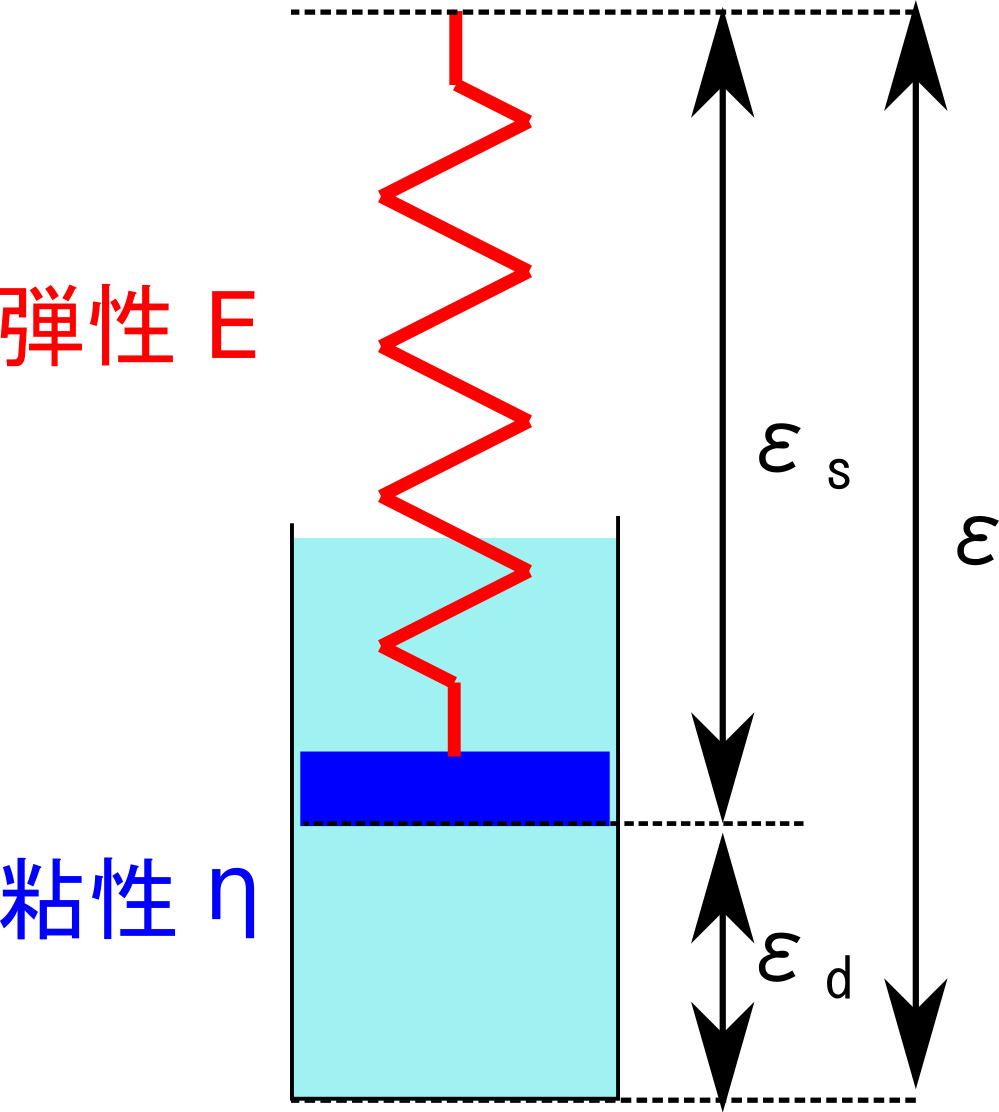
\includegraphics[width=\textwidth]{Maxwell_model.png}
		\end{columns}
\end{frame}

\begin{frame}
	\frametitle{マックスウェルモデル}
		\begin{columns}[T, onlytextwidth]
			\column{.5\linewidth}
				\begin{block}{マックスウェルモデルとは}
					\begin{itemize}
						\item 弾性モデル
						\begin{align*}
							\sigma_s(t) = E \varepsilon_s(t)
						\end{align*}
						\item 粘性モデル
						\begin{align*}
							\sigma_d(t) = \eta \dfrac{\mathrm{d}}{\mathrm{d}t}\varepsilon_d(t)
						\end{align*}
						\item 直列に連結だから、
						\begin{itemize}
							\item 応力は共通
						\item ひずみはそれぞれの和
						\end{itemize}
					\end{itemize}		
				\end{block}
			\column{.45\linewidth}
				\vspace{3mm}
				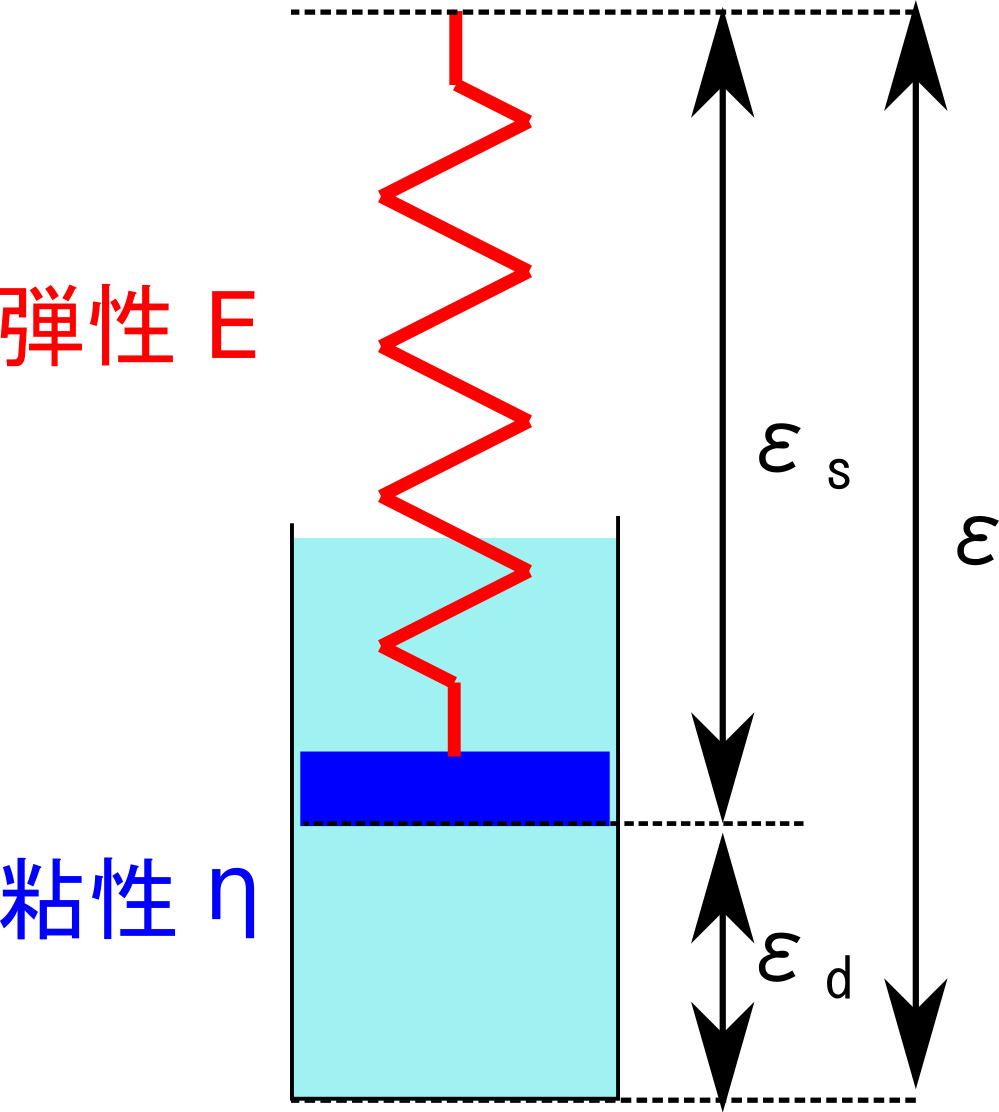
\includegraphics[width=.8\textwidth]{Maxwell_model.png}
				% \vspace{-3mm}
				\begin{align*}
					\begin{cases}
						\sigma = \sigma_s = \sigma_d \\
						\varepsilon = \varepsilon_s + \varepsilon_d
					\end{cases}
				\end{align*}
		\end{columns}
\end{frame}

\begin{frame}
	\frametitle{マックスウェルモデルの方程式}
		\small
		$\varepsilon = \varepsilon_s + \varepsilon_d$ を微分して、
		\begin{align*}
			\dfrac{\mathrm{d}}{\mathrm{d}t}\varepsilon = \dfrac{\mathrm{d}}{\mathrm{d}t}\varepsilon_s + \dfrac{\mathrm{d}}{\mathrm{d}t}\varepsilon_d
		\end{align*}
		
		一方、弾性モデルの $\sigma_s(t) = E \varepsilon_s(t)$ を微分して、
		\begin{align*}
			\dfrac{\mathrm{d}}{\mathrm{d}t}\sigma = E \dfrac{\mathrm{d}}{\mathrm{d}t}\varepsilon_s
		\end{align*}

		これらを、粘性モデルの $\sigma_d(t) = \eta \dfrac{\mathrm{d}}{\mathrm{d}t}\varepsilon_d(t)$ に代入して、以下の微分方程式として、\alert{マックスウェルの方程式}を得る。
		\color{red}
		\begin{align*}
			\dfrac{\mathrm{d}\varepsilon}{\mathrm{d}t} = \dfrac{1}{E} \dfrac{\mathrm{d}\sigma}{\mathrm{d}t} + \dfrac{\sigma}{\eta}
		\end{align*}
\end{frame}

\subsection{応力緩和}
\begin{frame}
	\frametitle{応力緩和}
		\begin{columns}[T, onlytextwidth]
			\column{.48\linewidth}
				\begin{block}{マクロには}
					\begin{itemize}
						\item 物質に、(瞬間的に)ひずみを与えて、
						\item その状態に維持。
						\item 応力が次第に減少。
					\end{itemize}
				\end{block}
			\column{.48\linewidth}
			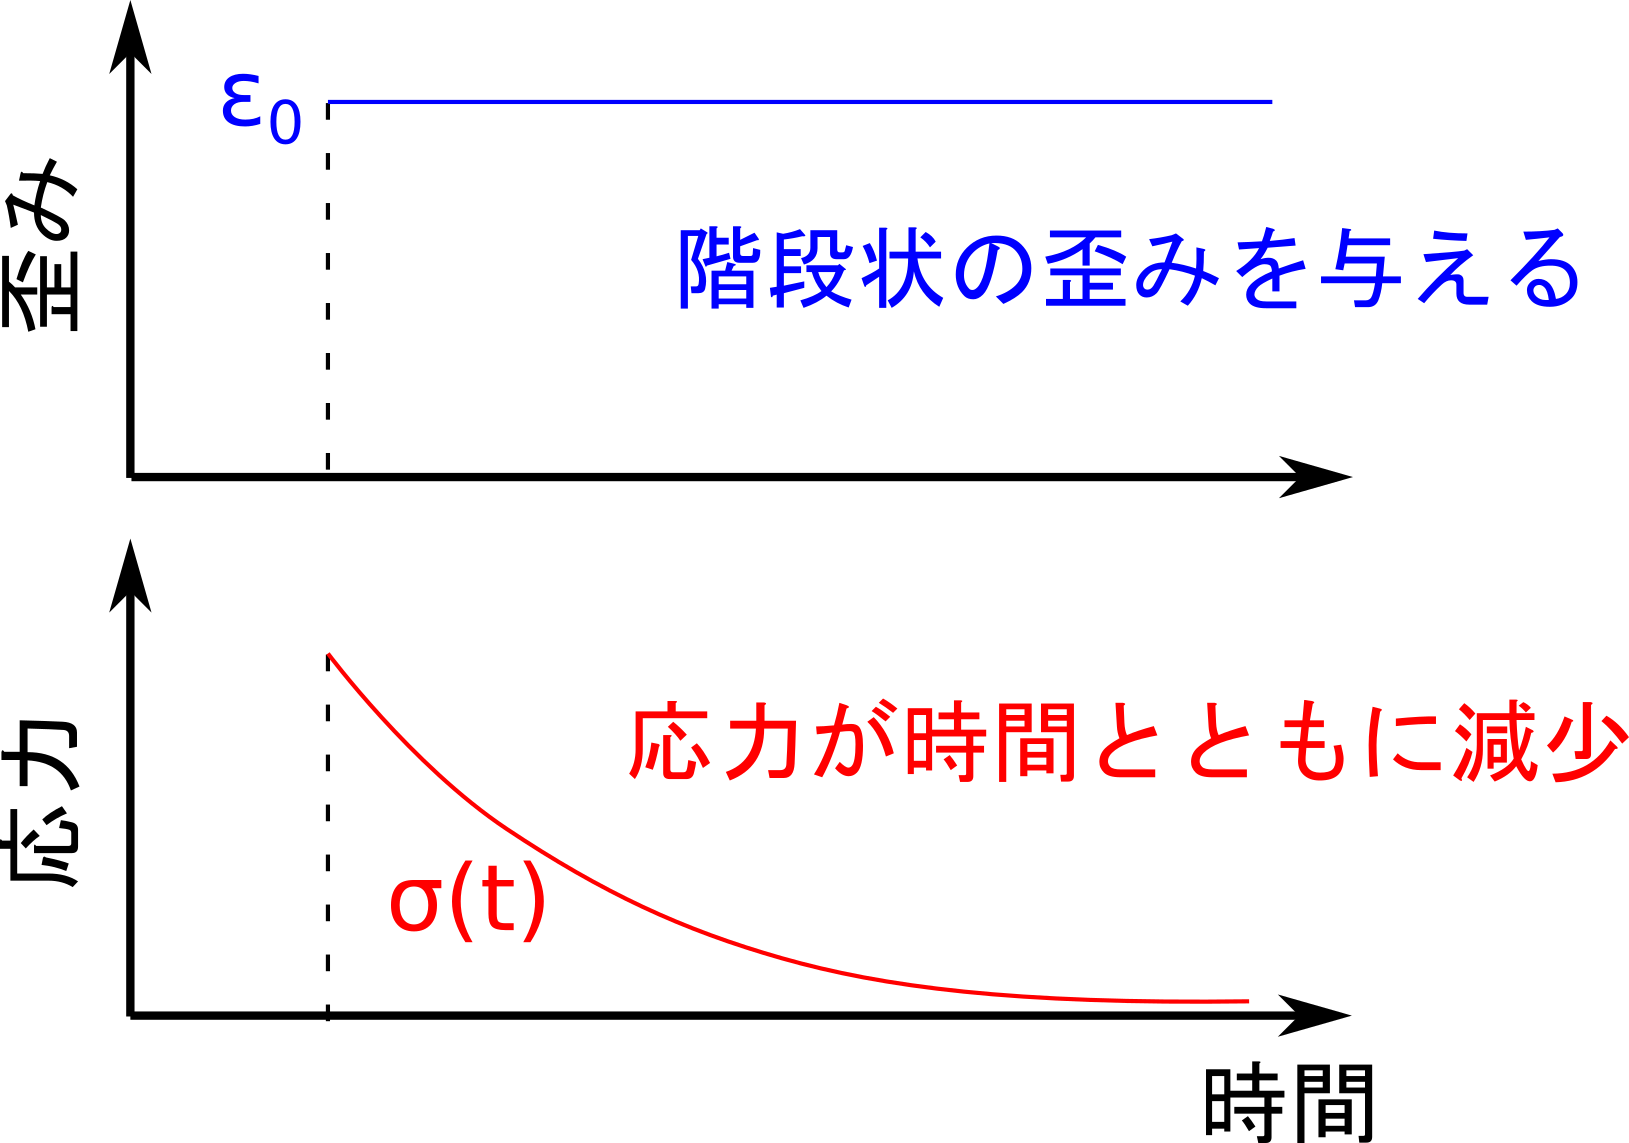
\includegraphics[width=\textwidth]{stress_relux.png}
		\end{columns}
		
		\begin{exampleblock}{ミクロには}
			\begin{itemize}
				\item 居心地のいい状態にいた粒子が、突然、居心地が変化。
				\item 少しずつ、\alert{居心地を改善}していく。
				\item 局所的な応力が消失。
			\end{itemize}
		\end{exampleblock}
\end{frame}

\begin{frame}
	\frametitle{マックスウェルモデルで応力緩和を}
		\begin{block}{数式展開(途中まで)}
			応力緩和ではひずみ一定(ひずみの微分が 0)なので、$\dfrac{\mathrm{d}}{\mathrm{d}t}\varepsilon =0$ をマックスウェル方程式に代入して、
			\begin{align*}
				&\dfrac{1}{E} \dfrac{\mathrm{d}\sigma}{\mathrm{d}t} + \dfrac{\sigma}{\eta} = 0 \\
				&\dfrac{\mathrm{d}\sigma}{\mathrm{d}t} = -\dfrac{E}{\eta} \sigma \;\; \text{\structure{(上式の第一項を右辺に移行)}}\\
				&{\color{red}\int \dfrac{1}{\sigma} \mathrm{d}\sigma} = -\dfrac{E}{\eta}  {\color{red} \int \mathrm{d}t} \; \;\text{\structure{(変数を振り分けてから、両辺を積分)}}\\
				&{\color{red}\ln \sigma} = -\dfrac{E}{\eta} {\color{red}t} + C \;\; \text{\structure{(\alert{積分の公式}に従い、積分定数を追加)}}
			\end{align*}
		\end{block}
\end{frame}

\begin{frame}
	\frametitle{マックスウェルモデルで応力緩和を}
		\begin{block}{数式展開(続き)}
			$t=0$ での初期応力を $\sigma_0$ とすると、$C=\ln \sigma_0$ となり、
			\vspace{-2mm}
			\begin{align*}
				&\ln \sigma = -\dfrac{E}{\eta} t + \ln \sigma_0 \\
				&\ln \sigma - \ln \sigma_0 = -\dfrac{E}{\eta} t \\
				&\ln \dfrac{\sigma}{\sigma_0} = -\dfrac{E}{\eta} t \;\; \text{\structure{(対数の引き算は、真数の割り算)}}
			\end{align*}

			対数を指数に変換して、$\tau = \dfrac{\eta}{E}$ と書き換えて、
			\vspace{-2mm}
			\begin{align*}
				\sigma(t) = \sigma_0 \exp \left(-\dfrac{E}{\eta} t \right) = \sigma_0 \exp \left(-\dfrac{t}{\tau} \right)
			\end{align*}
		\end{block}
\end{frame}

\begin{frame}
	\frametitle{応力緩和の挙動}
		\begin{columns}[T, onlytextwidth]
			\column{.48\linewidth}
				\begin{exampleblock}{指数関数的減少とは?}
					\begin{itemize}
						\item 下式をグラフに表すと、右図となる。
						\begin{align*}
							\sigma(t) = \sigma_0 \exp \left(-\dfrac{t}{\tau} \right)
						\end{align*}
						\item 時間経過に伴い応力が減少し $t = \tau$ において
						\begin{align*}
							\sigma(\tau) 
							&= \sigma_0 \exp(-1)\\ 
							&= \dfrac{\sigma_0}{e}
						\end{align*}
					\end{itemize}
				\end{exampleblock}
			\column{.48\linewidth}
				\begin{alertblock}{緩和時間とは、}
					時間の次元を持つ $\tau$ は、初期の $\dfrac{1}{e}$ となる時間
				\end{alertblock}
				\begin{center}
					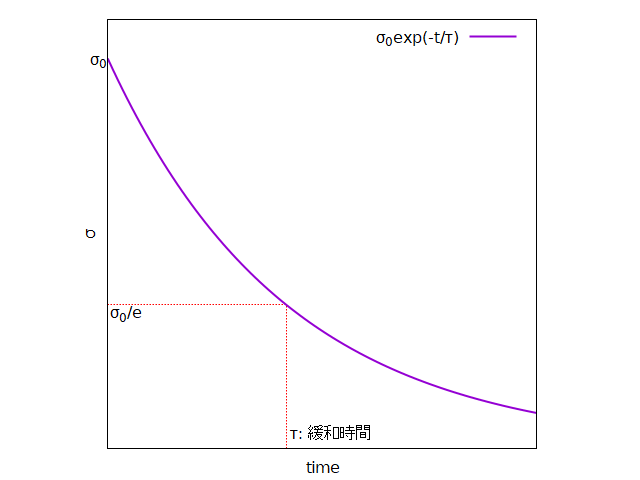
\includegraphics[width=\textwidth]{relux_3.png}
				\end{center}
		\end{columns}
\end{frame}

\subsection{緩和時間}
\begin{frame}
	\frametitle{緩和時間}
		\begin{align*}
			\text{(緩和時間)}\;\tau = \dfrac{\eta}{E}\; \left( \dfrac{\text{粘度}}{\text{弾性率}} \right)
		\end{align*}
		\vspace{-3mm}
		\begin{itemize}
			\item 緩和時間とは
			\begin{itemize}
				\item 弾性モデルにおける弾性率 $E$ の単位は Pa、
				\item 粘性モデルにおける粘度 $\eta$ の単位は Pa$\cdot$s、
				\item その比である $\tau$ は時間の次元 [T] を持ち、\\緩和時間と呼ばれる。
				\item 緩和時間とは、物質のひずみに対する力学応答が、\\指数関数的に減少するさまを表す特徴的な時間。
			\end{itemize}
			\item 緩和時間の振る舞い
			\begin{itemize}
				\item 弾性応答の性質を表す弾性率に反比例し、
				\item 粘性応答の度合いを表す粘度に比例する。
			\end{itemize}
		\end{itemize}
\end{frame}

\begin{frame}
	\frametitle{緩和挙動のイメージ}
		\begin{alertblock}{プロットのヒント}
			\begin{itemize}
				\item 軸のスケールで見た目のイメージは変る。
			\end{itemize}
		\end{alertblock}
		\begin{columns}[T, onlytextwidth]
			\column{.48\linewidth}
				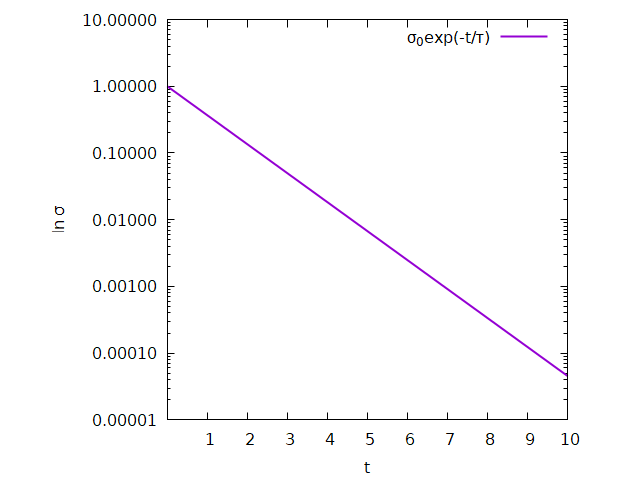
\includegraphics[width=\textwidth]{relux_4.png}
				片対数グラフ:傾きが緩和時間に対応
			\column{.48\linewidth}
				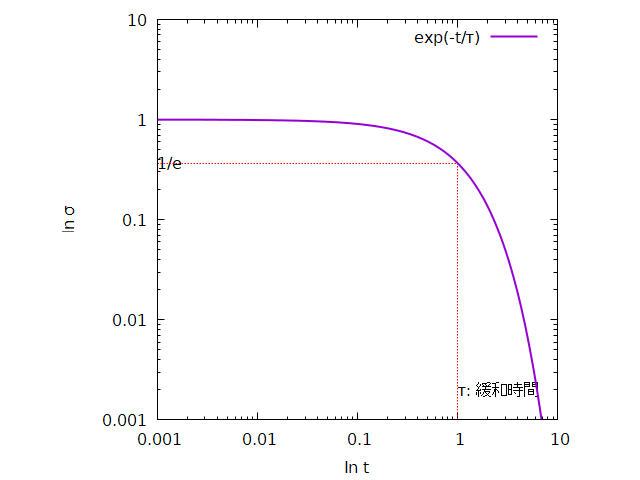
\includegraphics[width=\textwidth]{relux_5.png}
				両対数グラフ:緩和時間近傍で応力が急激に低下
		\end{columns}
\end{frame}

\begin{frame}
	\frametitle{緩和時間が異なると}
		\begin{alertblock}{緩和時間の異なるものを比較}
			\begin{itemize}
				\item 軸のスケールで見た目のイメージは変る。
			\end{itemize}
		\end{alertblock}
		\begin{columns}[T, onlytextwidth]
			\column{.48\linewidth}
				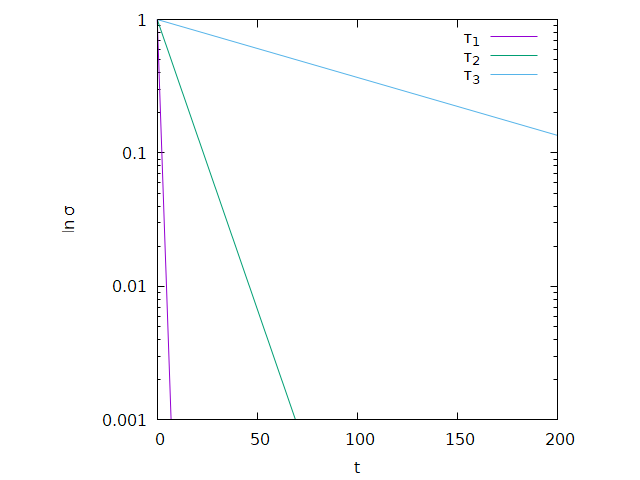
\includegraphics[width=\textwidth]{relux_6.png}
				片対数グラフ:傾きが緩和時間に対応
			\column{.48\linewidth}
				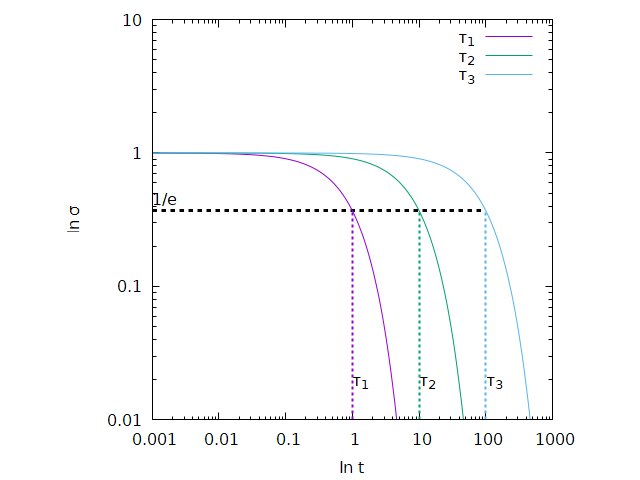
\includegraphics[width=\textwidth]{relux_7.png}
				両対数グラフ:緩和時間近傍で応力が急激に低下
		\end{columns}
\end{frame}

\section{少しだけ実事象に近づけると}
\subsection{複数の緩和時間}
\begin{frame}
	\frametitle{複数の緩和時間}
		\begin{columns}[T, onlytextwidth]
			\column{.5\linewidth}
			\begin{itemize}
				\item 実際の物質の内部は、\\大抵の場合、均一とは\\言えないことが多い。
				\item その結果として、マクロには複雑な緩和挙動を示す。
				\item \alert{仮想的}に、内部に\alert{複数の緩和時間}を考えよう。
				\item 右図のように\alert{モデル化}\\できる。
			\end{itemize}
			\column{.45\linewidth}
				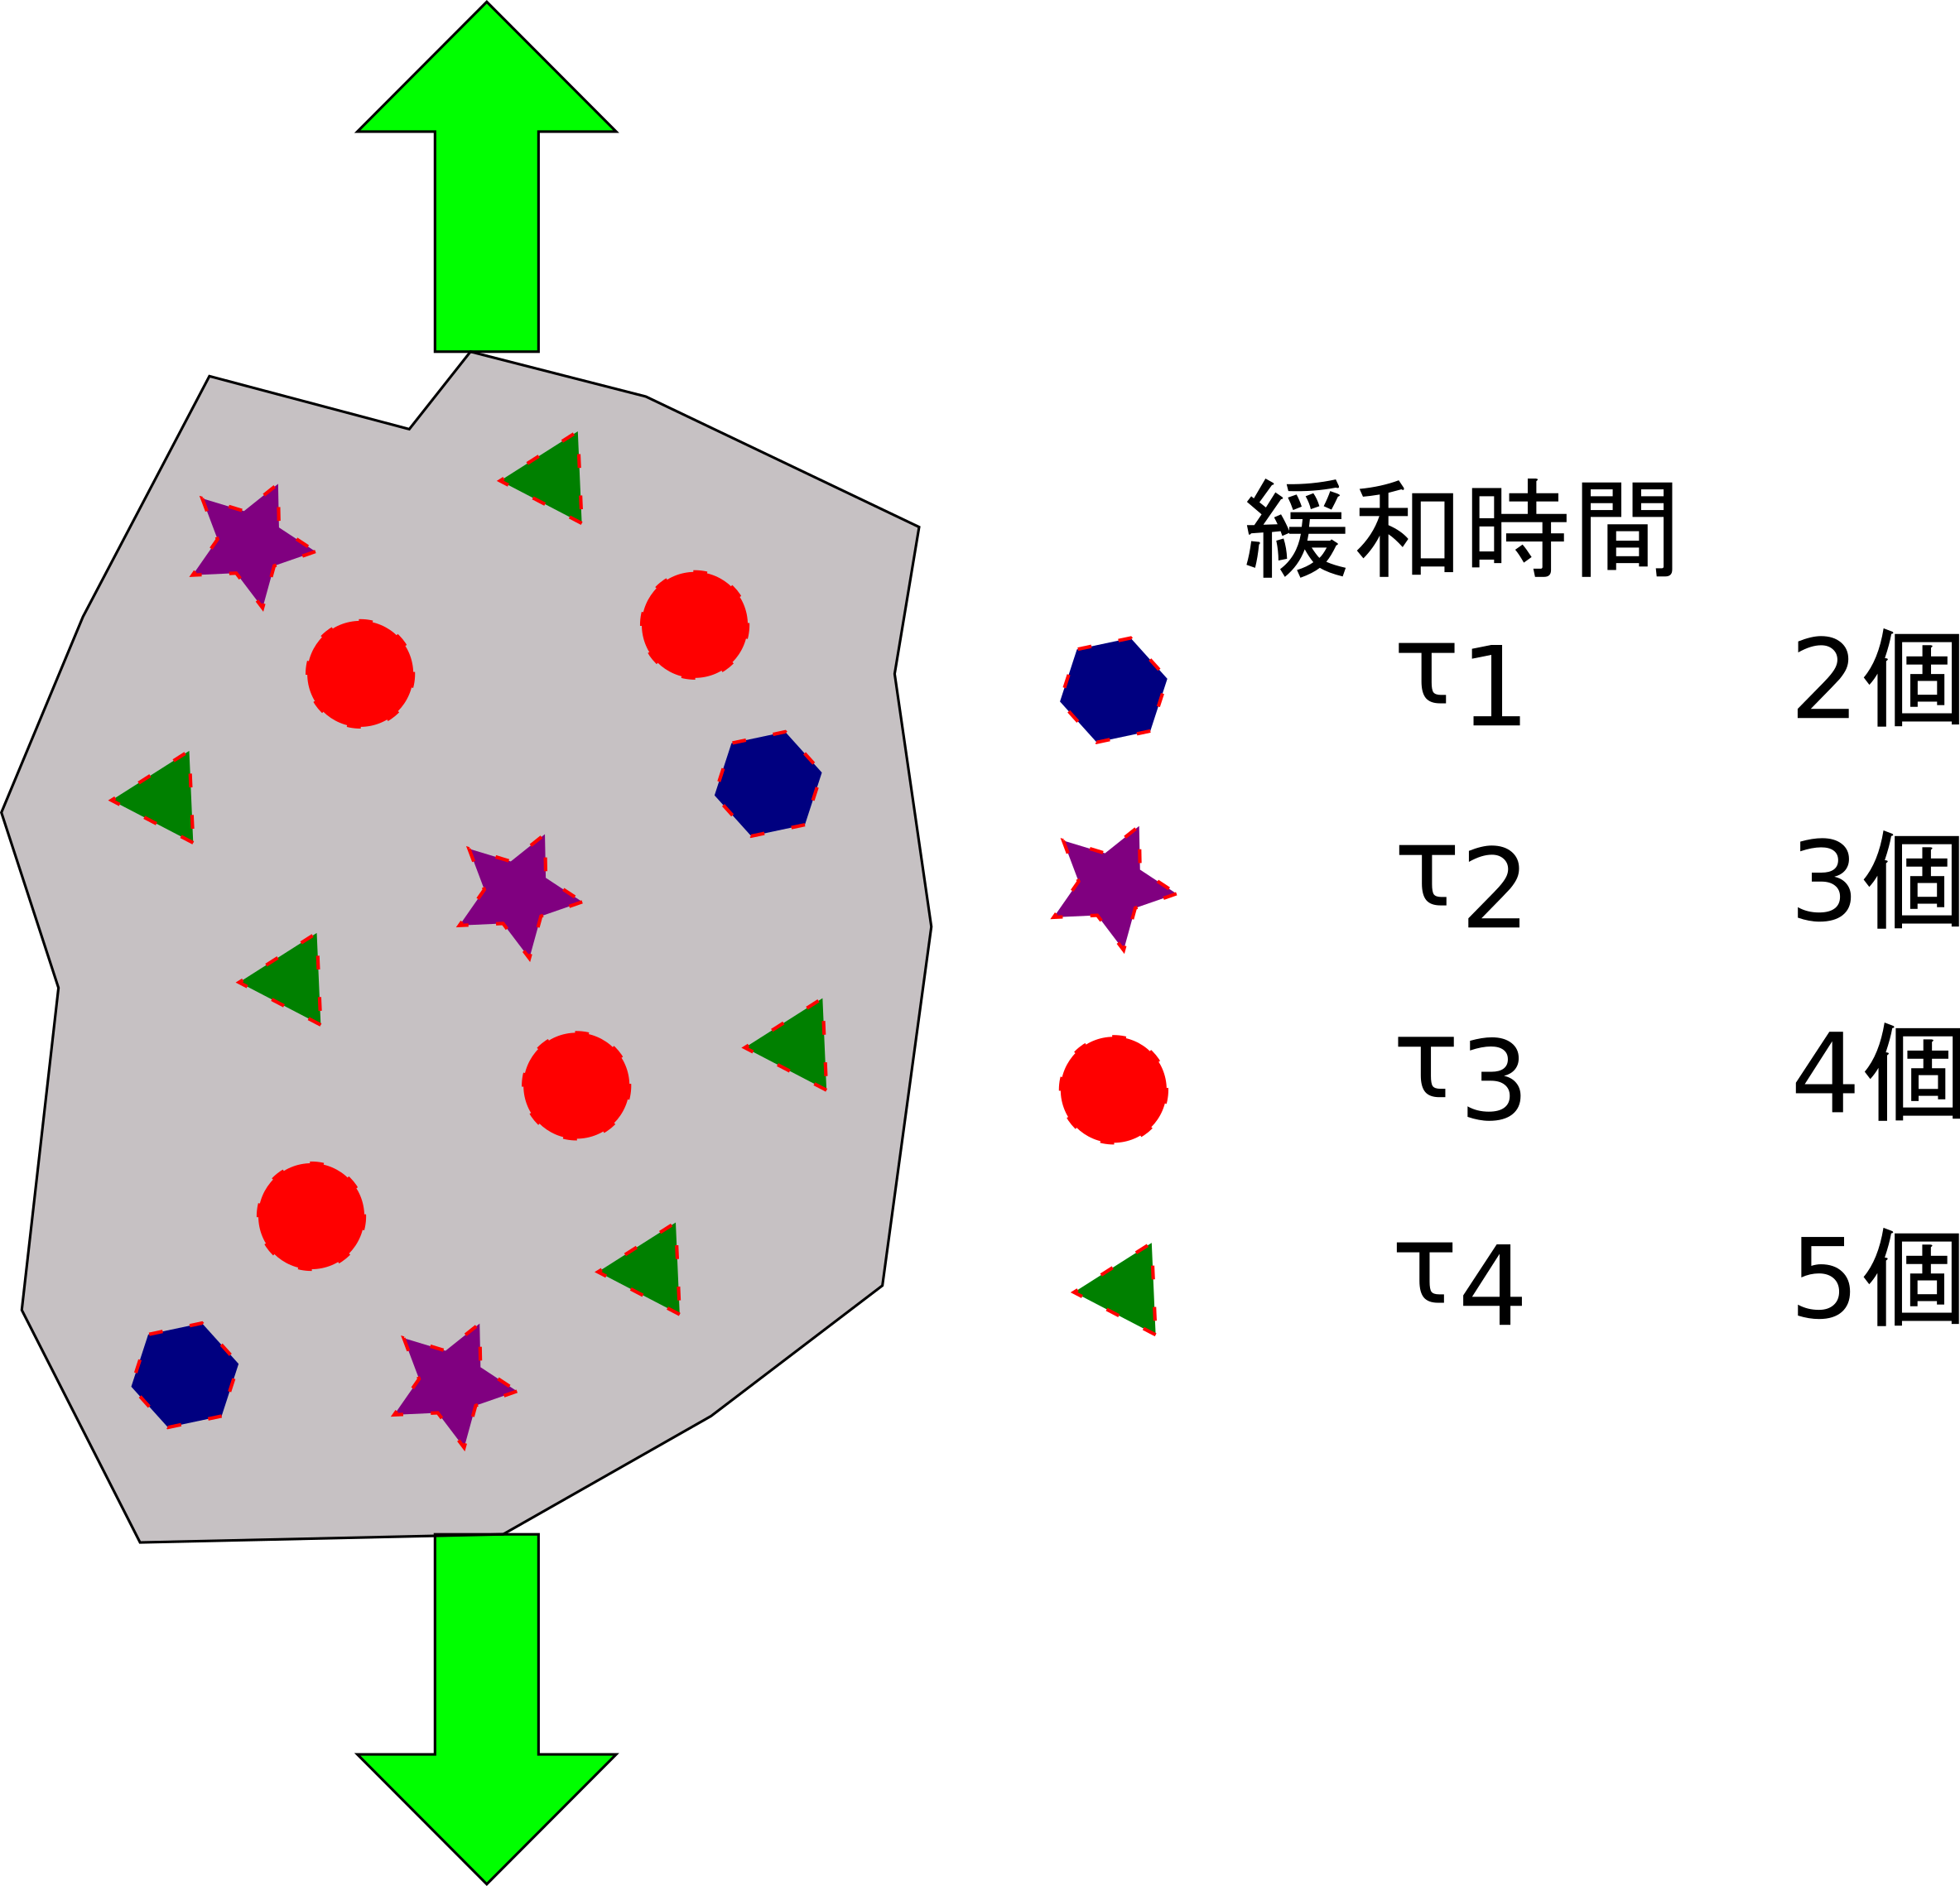
\includegraphics[width=\textwidth]{relux_multi.png}
		\end{columns}
\end{frame}

\subsection{一般化マックスウェルモデルについて}
\begin{frame}
	\frametitle{複数のマックスウェルモデル}
		\begin{block}{一般化マックスウェルモデル}
			\begin{itemize}
				\item \alert{それぞれの緩和時間に対応}するように、複数の\\マックスウェルモデルを想定し、
				\item すべてを、\alert{並列に連結}。
			\end{itemize}
		\end{block}
		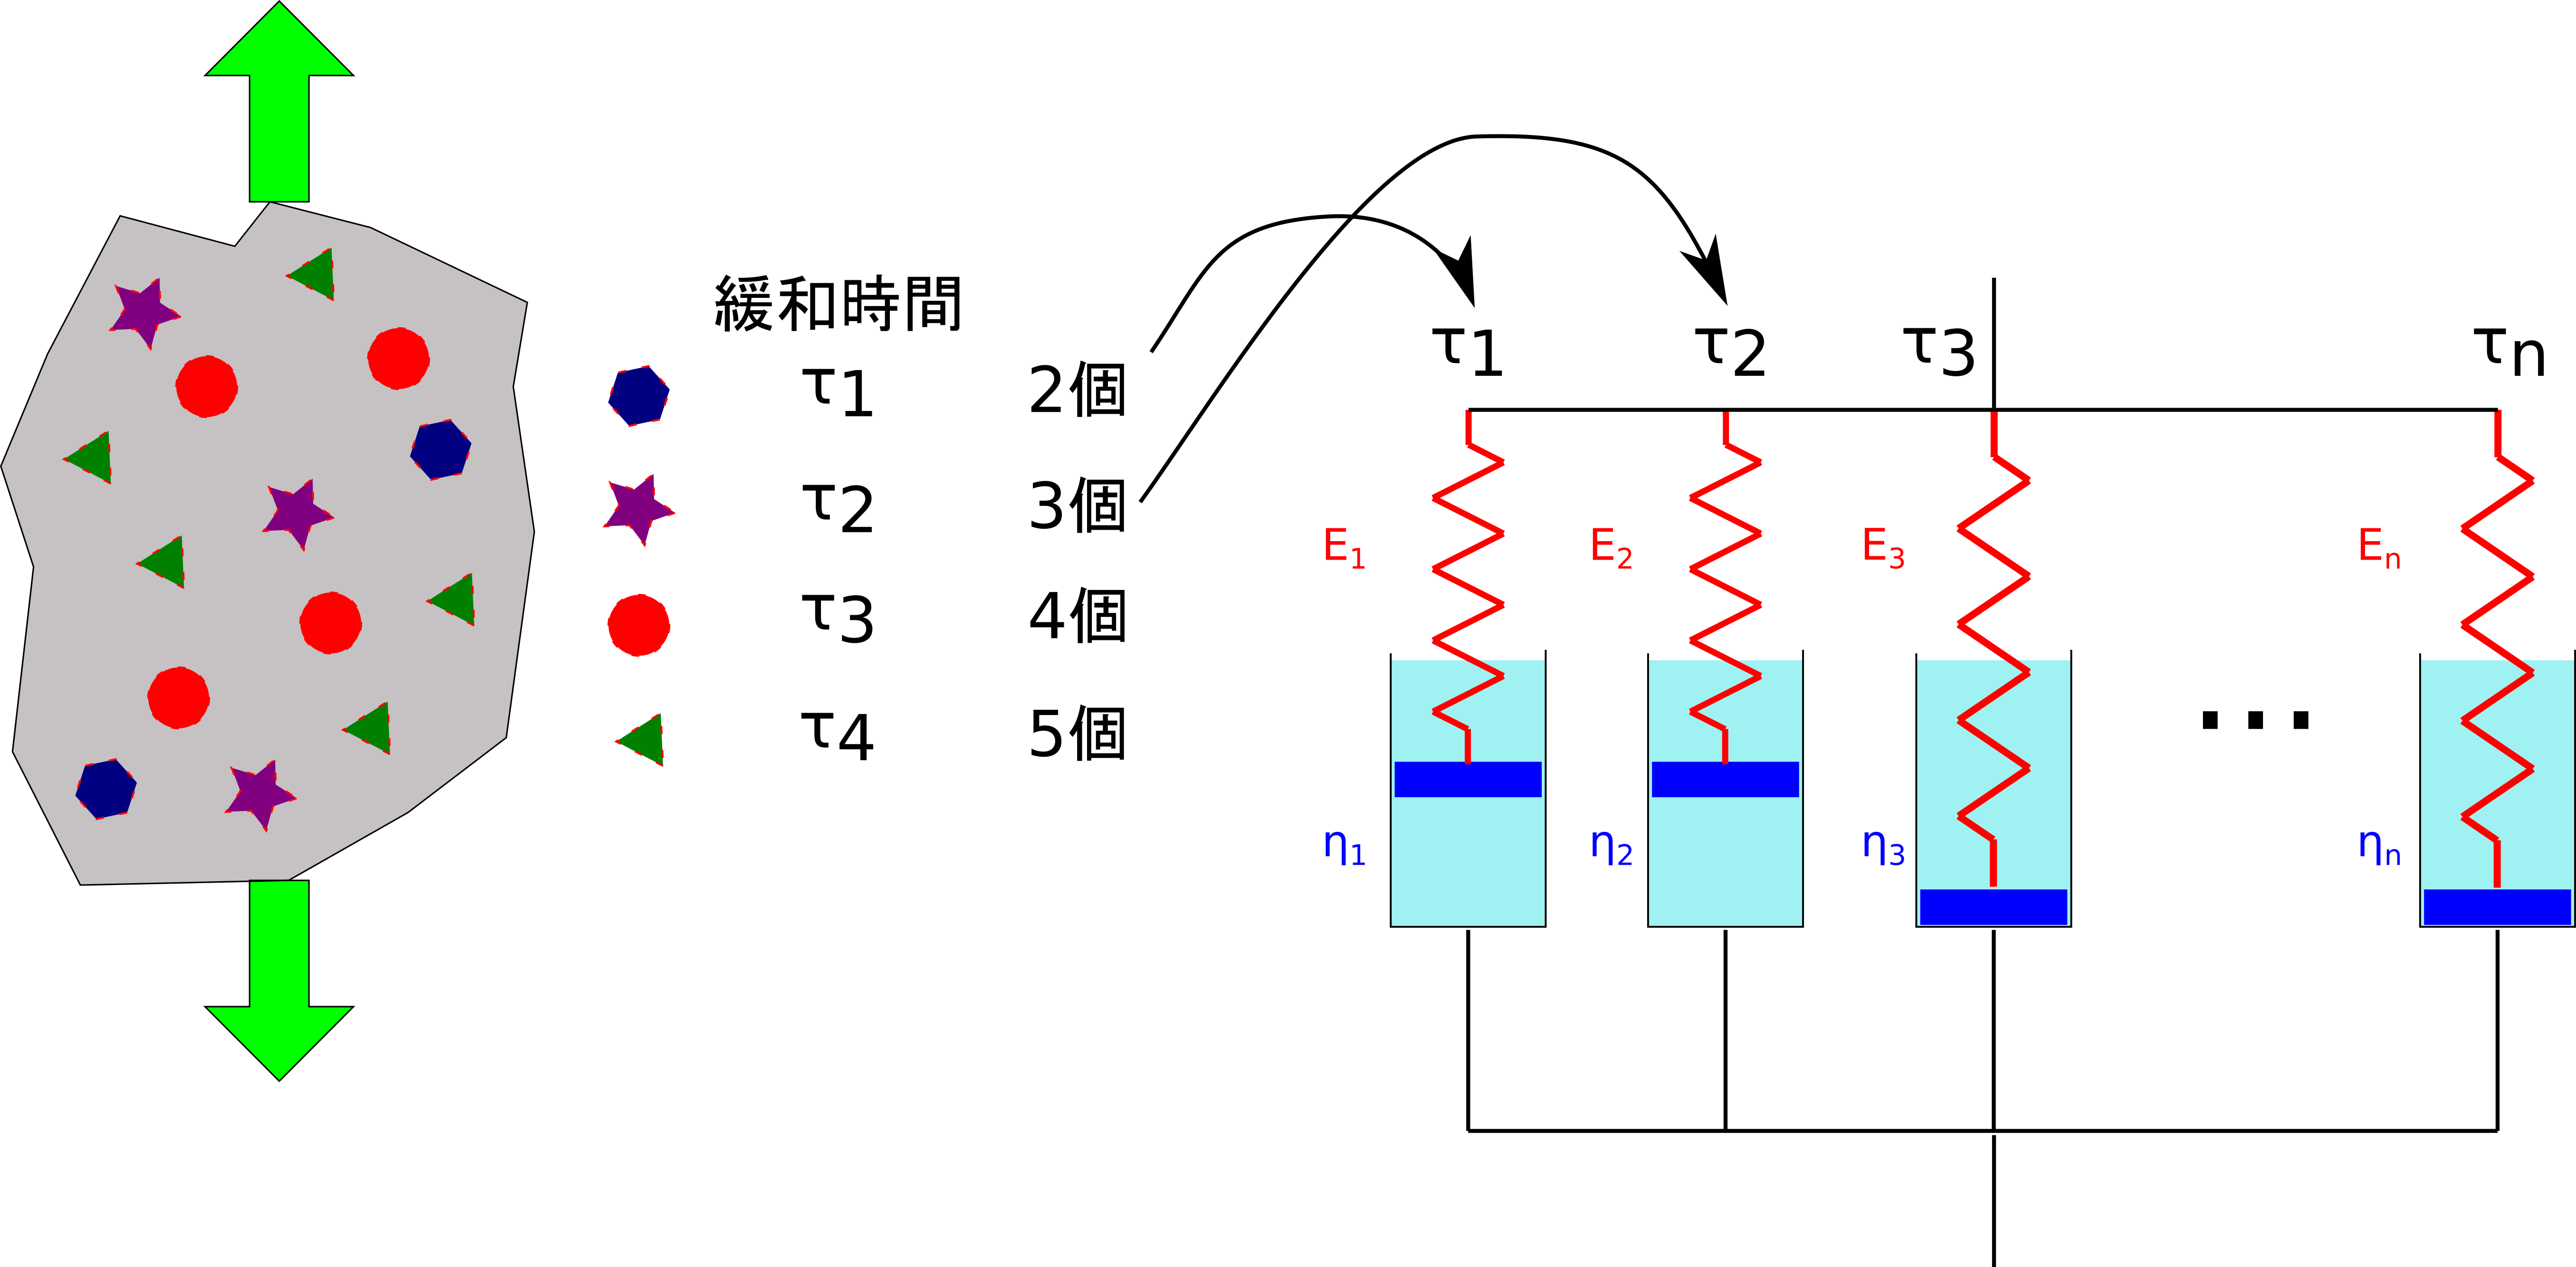
\includegraphics[width=\textwidth]{relux_multi_2.png}
\end{frame}

\begin{frame}
	\frametitle{一般化マックスウェルモデルの考え方}
		\begin{itemize}
			\item マックスウェルモデルを並列に連結したのだから、
			\begin{itemize}
				\item 応力はそれぞれのものの総和
				\begin{align*}
					\sigma = \sum_{i=1}^n \sigma_i
						= \sum_{i=1}^n \sigma_{0,i}\exp\left(-\dfrac{t}{\tau_i} \right)
				\end{align*}
				\item ひずみ $\varepsilon$ はそれぞれに共通なので、両辺を除して、
				\begin{align*}
					\dfrac{\sigma}{\varepsilon} &= \sum_{i=1}^n \dfrac{\sigma_{0,i}}{\varepsilon}\exp\left(-\dfrac{t}{\tau_i} \right) \\
					\therefore \; E(t) &= \sum_{i=1}^n E_i \exp\left(-\dfrac{t}{\tau_i} \right)
				\end{align*}
			\end{itemize}
			\item 結局、緩和時間の異なるそれぞれのモデルごとの、\\弾性率の緩和の総和とかける。
		\end{itemize}
\end{frame}

\begin{frame}
	\frametitle{緩和のイメージ}
		% 緩和時間の短いものから、順次緩和。
		\vspace{-5mm}
		\begin{columns}[T, onlytextwidth]
			\small
			\column{.46\linewidth}
				\begin{block}{初期状態}
					\begin{center}
						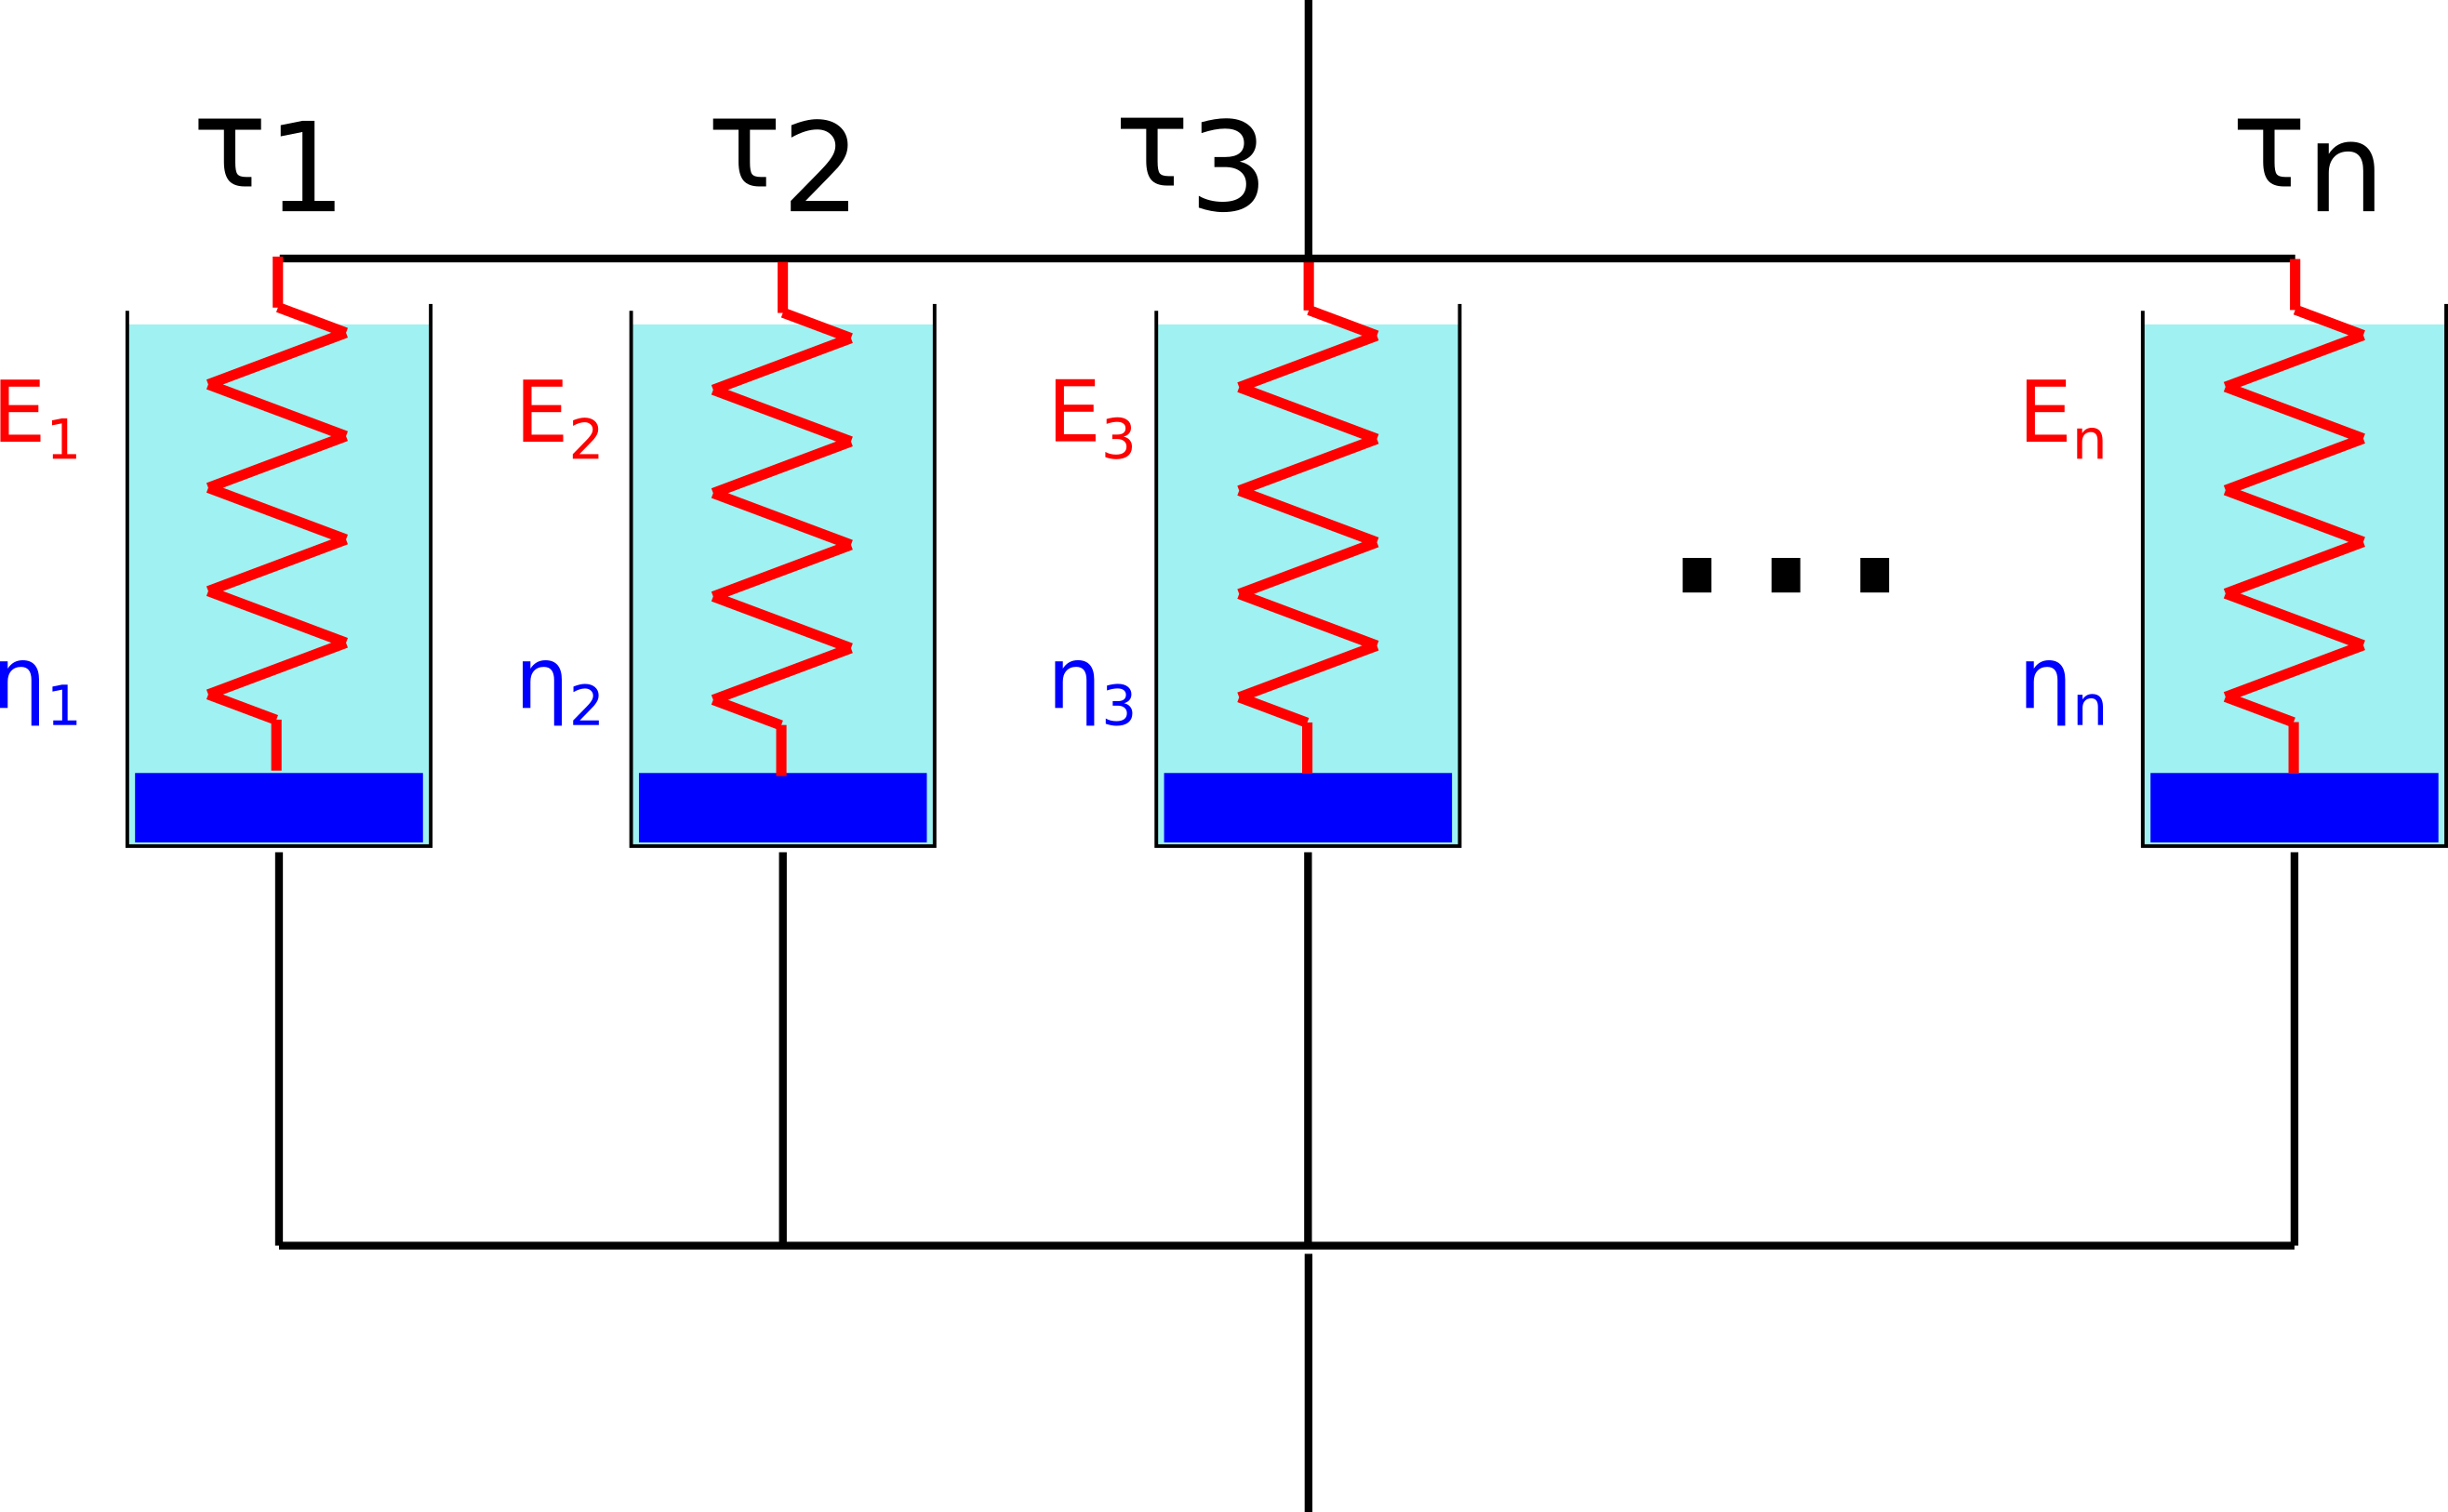
\includegraphics[width=.7\textwidth]{Maxwell_multi_0.png}
					\end{center}
				\end{block}
				\vspace{-3mm}
				\begin{block}<2->{変形直後}
					\begin{center}
						\includegraphics<2->[width=.7\textwidth]{Maxwell_multi_1.png}
					\end{center}
				\end{block}
			\column{.46\linewidth}
				\begin{block}<3->{$t>\tau_1$ 経過後}
					\begin{center}
						\includegraphics<3->[width=.7\textwidth]{Maxwell_multi_2.png}
					\end{center}
				\end{block}
				\vspace{-3mm}
				\begin{block}<4->{$t>\tau_2$ 経過後}
					\begin{center}
						\includegraphics<4->[width=.7\textwidth]{Maxwell_multi_3.png}
					\end{center}
				\end{block}
		\end{columns}
\end{frame}

\begin{frame}
	\frametitle{緩和のプロット}
		\begin{alertblock}{一般化マックスウェルの緩和挙動}
			\begin{itemize}
				\item 個々のマックスウェルモデルの緩和挙動の和となる。
				\item 仮に緩和強度が同一とすると、右図のように和となる。
				\item 時間経過に従い、順次緩和。
			\end{itemize}
		\end{alertblock}
		\begin{columns}[T, onlytextwidth]
			\column{.48\linewidth}
				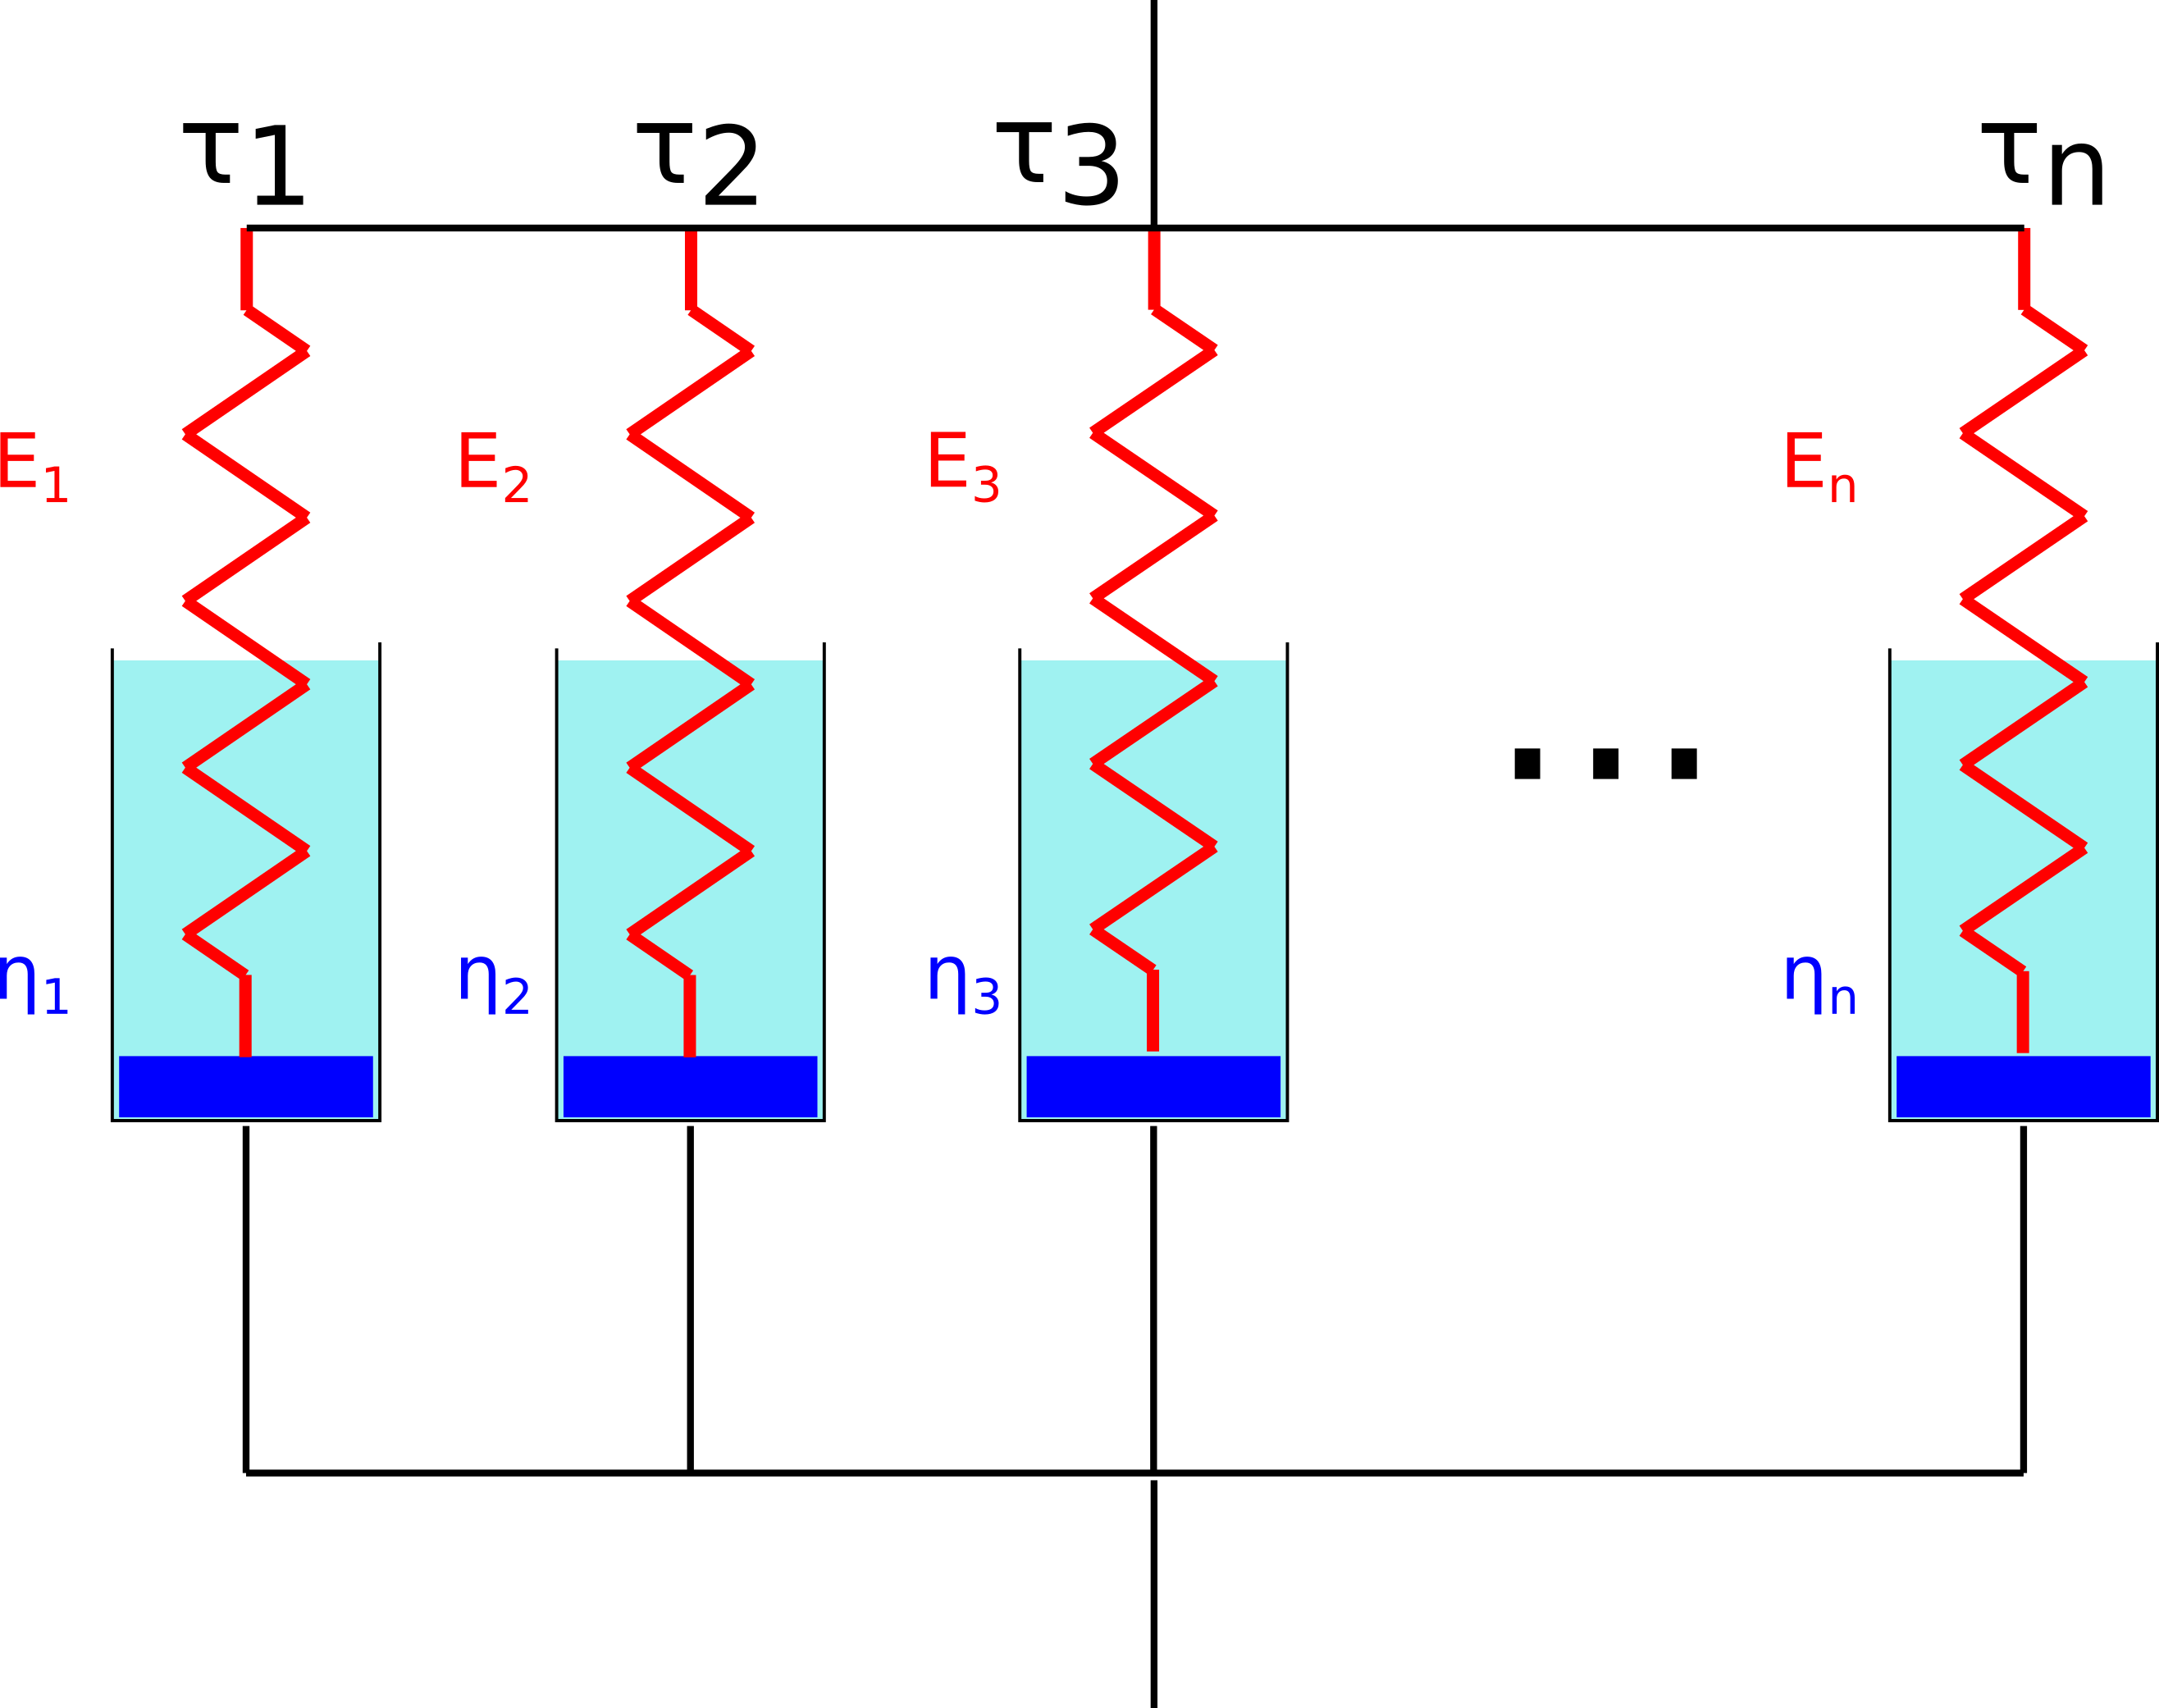
\includegraphics[width=\textwidth]{Maxwell_multi_1.png}
			\column{.48\linewidth}
				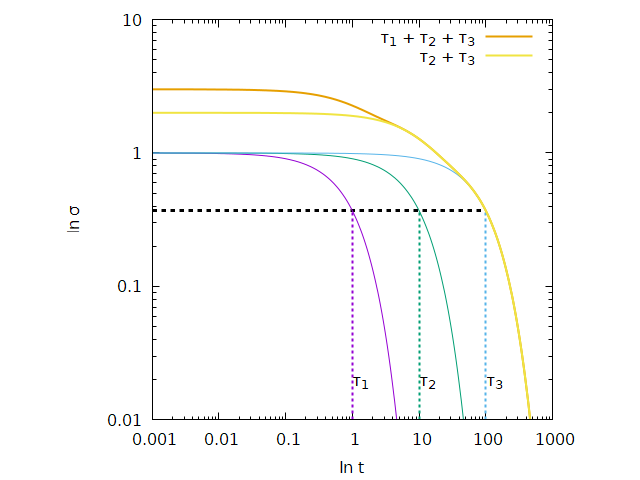
\includegraphics[width=\textwidth]{relux_8.png}
		\end{columns}
\end{frame}

\begin{frame}
	\frametitle{緩和のプロット}
		\begin{alertblock}{一般化マックスウェルの緩和挙動}
			\begin{itemize}
				\item 個々のマックスウェルモデルの緩和挙動の和となる。
				\item 仮に緩和強度が同一とすると、右図のように和となる。
				\item 時間経過に従い、順次緩和。
			\end{itemize}
		\end{alertblock}
		\begin{columns}[T, onlytextwidth]
			\column{.48\linewidth}
				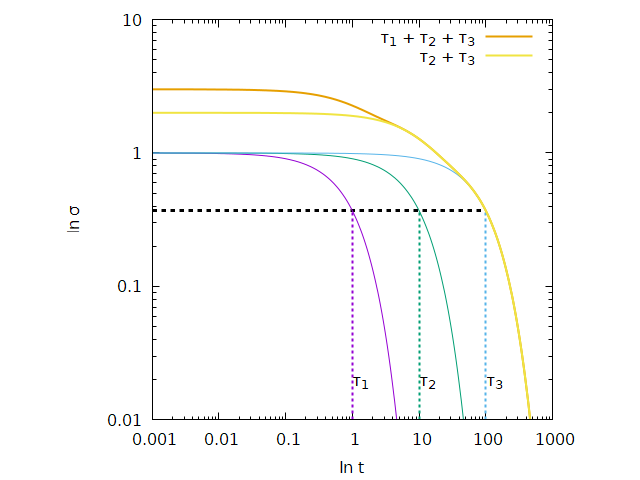
\includegraphics[width=\textwidth]{relux_8.png}
			\column{.48\linewidth}
				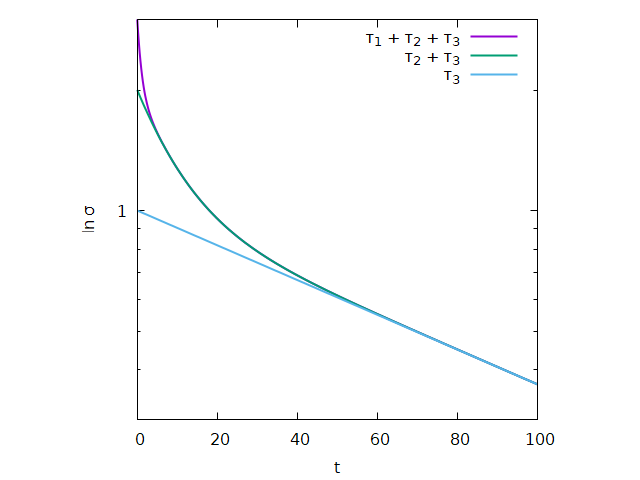
\includegraphics[width=\textwidth]{relux_9.png}
		\end{columns}
\end{frame}

\subsection{応力緩和で見た固体と液体}
\begin{frame}
	\frametitle{応力緩和で見た固体と液体}
		\begin{columns}[T, onlytextwidth]
			\column{.48\linewidth}	
				\begin{block}{粘弾性体の特徴}
					\begin{itemize}
						\item ステップひずみの
						\item 長時間の緩和において、
						\item $E \rightarrow 0$\\
						流動する粘弾性液体
						\item 固体は緩和しない成分が残存
					\end{itemize}
				\end{block}
			\column{.48\linewidth}
				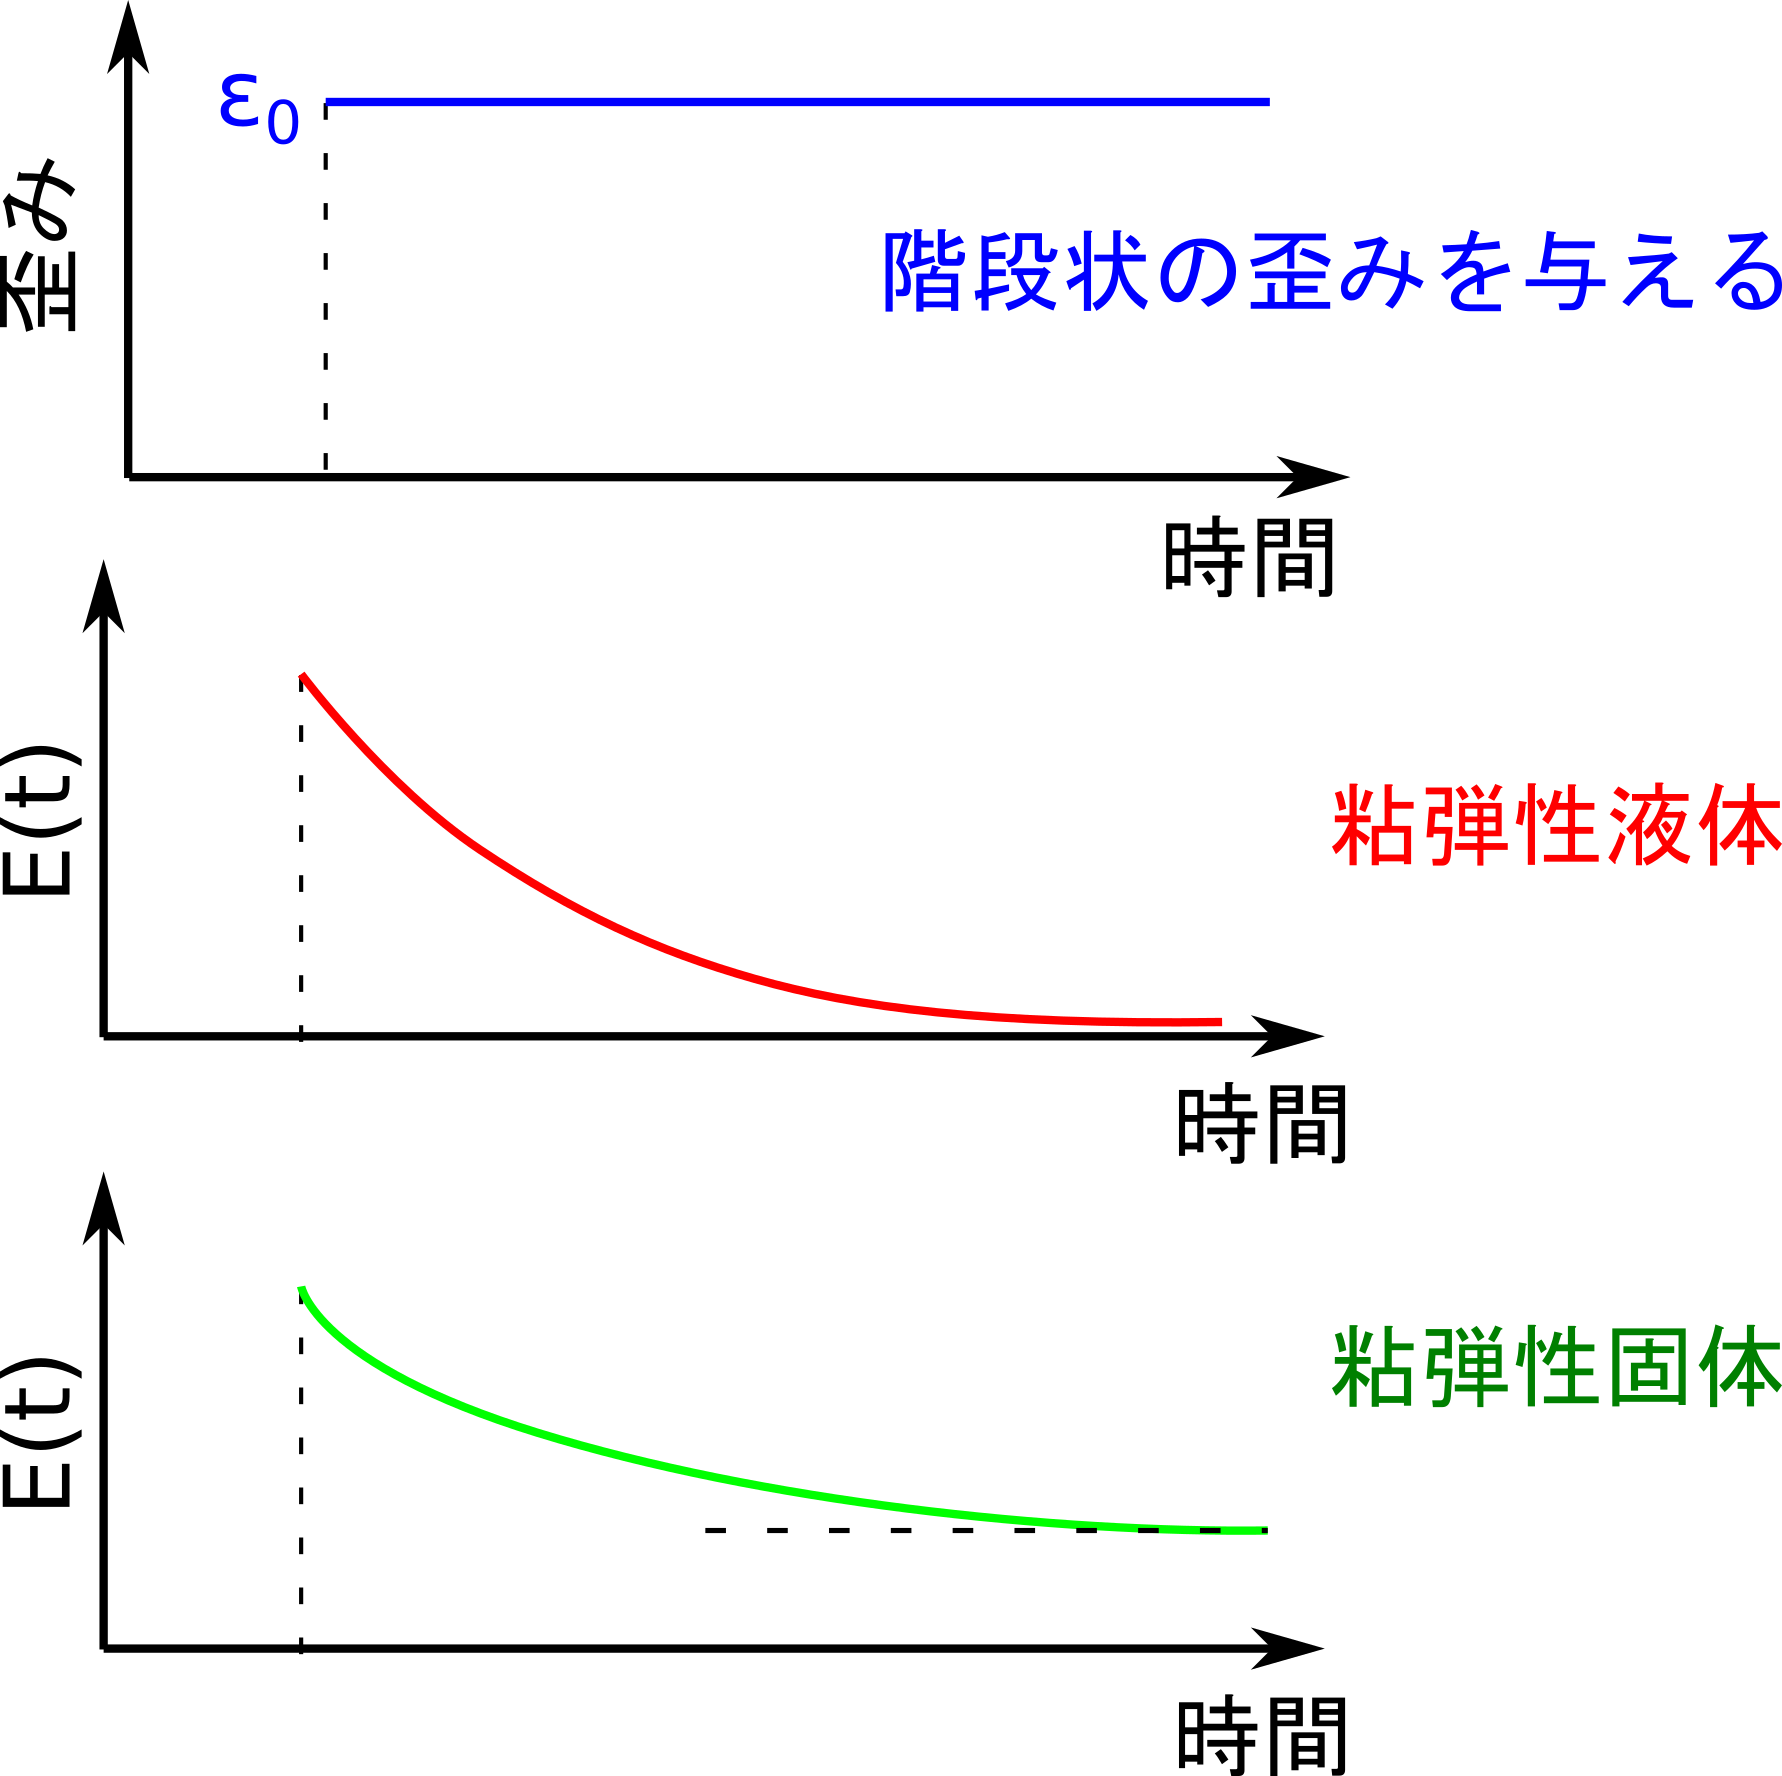
\includegraphics[width=\textwidth]{stress_solid_liquid.png}
		\end{columns}
\end{frame}

\begin{frame}
	\frametitle{まとめ}
        \begin{boxnote}
            \vspace{-3mm}
            \begin{itemize}
                \item 粘性と弾性についての再確認
                    \begin{itemize}
                        \item 固体と液体の応答について振り返り、
                        \item その組み合わせとして粘弾性
                    \end{itemize} 
                \item 粘弾性のモデル化
                    \begin{itemize}
                        \item 粘弾性の単純なモデルをつくって、
                        \item 応力緩和と緩和時間
                    \end{itemize} 
                \item 少しだけ実事象に近づけると
                    \begin{itemize}
                        \item 複数の緩和時間を一般化マックスウェルモデル
                        \item 応力緩和で見た固体と液体
                    \end{itemize}
            \end{itemize}
        \end{boxnote}
\end{frame}

% \appendix
% \backupbegin

% \section{演習問題 1}
% \subsection{「粘性と弾性についての再確認」}
% \begin{frame}
% 	\frametitle{「粘性と弾性についての再確認」}
% 	\small
% 		\begin{itemize}
% 			\item \textcolor<2>{black}{固体}のモデルでは応力は\fbox{\textcolor<1>{white}{ひずみ}}に比例し、液体のモデルでは応力は\fbox{\textcolor<1>{white}{ひずみ速度}}に比例します。
% 			\item 固体では\fbox{\textcolor<1>{white}{時間}}に関係なく力の釣り合いで考えることができ、液体では\fbox{\textcolor<1>{white}{時間の因子}}が重要になります。
% 		\end{itemize}
% \end{frame}

% \backupend
\end{document}